%!TEX root = ../template.tex
%%%%%%%%%%%%%%%%%%%%%%%%%%%%%%%%%%%%%%%%%%%%%%%%%%%%%%%%%%%%%%%%%%%
%% chapter2.tex
%%%%%%%%%%%%%%%%%%%%%%%%%%%%%%%%%%%%%%%%%%%%%%%%%%%%%%%%%%%%%%%%%%%

\typeout{NT FILE chapter2.tex}%

\chapter{Background}
\label{cha:background}

%%------------------------------------------------------------
%% SECTION: Foundations of Neural Language Representation
%%------------------------------------------------------------
\section{Foundations of Neural Language Representation}
\label{sec:foundations}

Representing language in a machine-processable form is a prerequisite for any
modern Generative AI system. Two landmark contributions established the
foundations upon which contemporary large language models (LLMs) and
retrieval-augmented architectures are built: dense word representations learned
via neural networks, and the Transformer architecture based solely on attention.

\subsection{Distributed Word Representations}
\label{sec:word2vec}

Prior to 2013, natural language processing relied predominantly on sparse,
high-dimensional representations such as one-hot encodings, which offered no
intrinsic notion of semantic similarity. Mikolov et
al.~\cite{mikolov2013word2vec} addressed this with Word2Vec, an efficient
framework for learning continuous vector representations of words from large
unlabelled corpora. The model is trained through a self-supervised prediction
task using one of two architectures: Continuous Bag-of-Words (CBOW), which
predicts a target word from its context, or Skip-gram, which performs the
inverse prediction.

\begin{figure}[htbp]
    \centering
    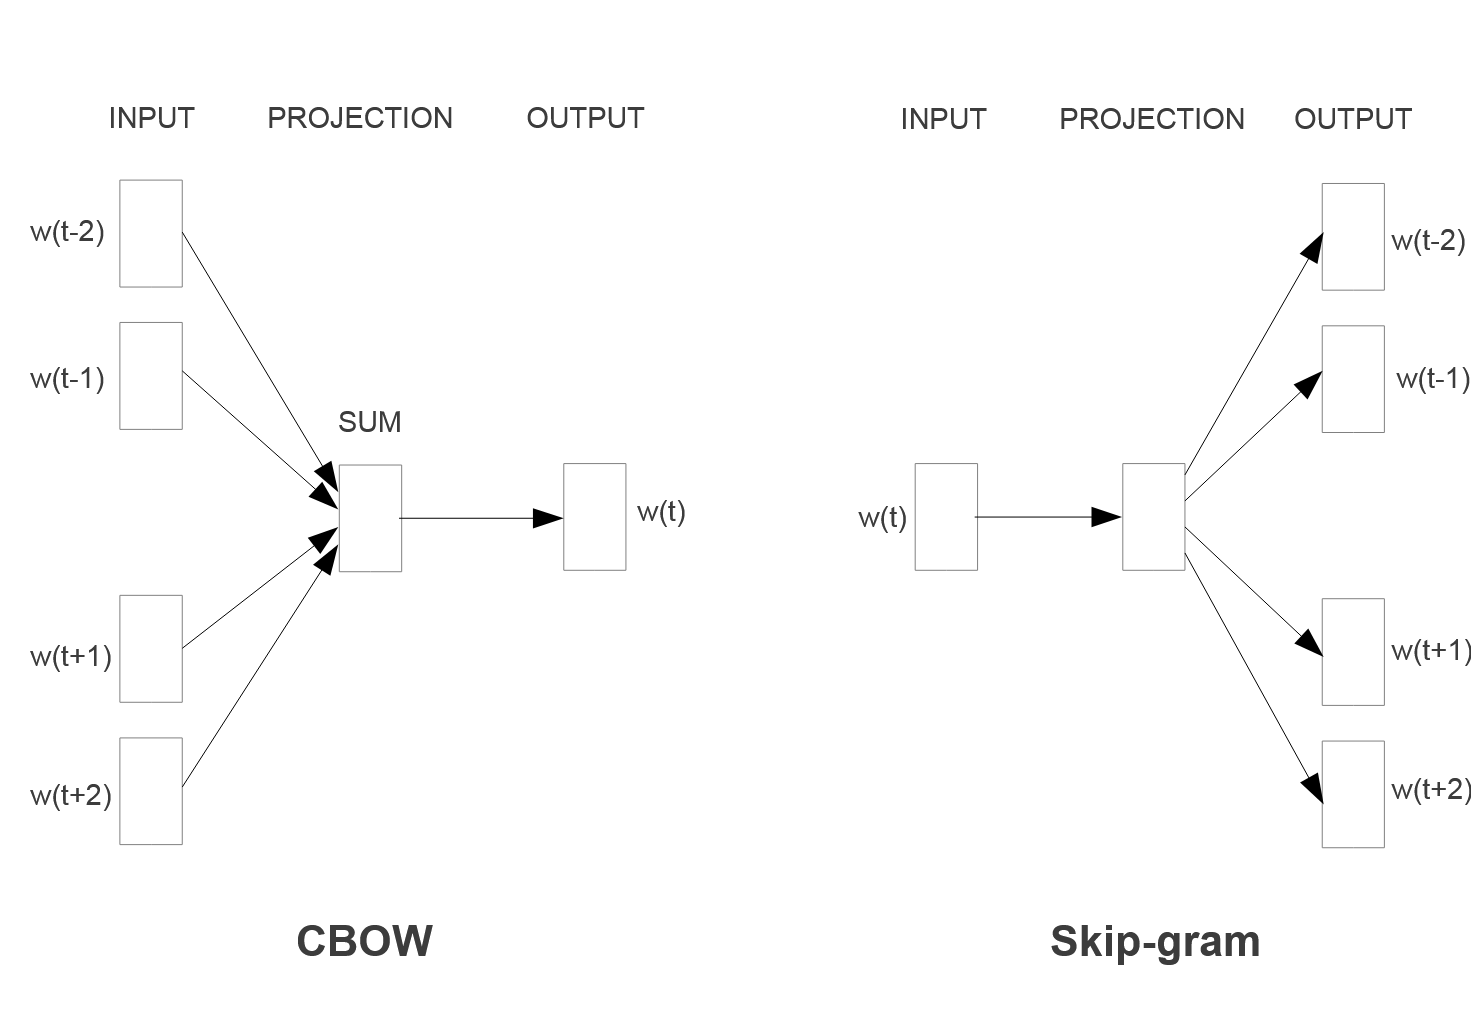
\includegraphics[width=0.85\textwidth]{5-Figures/Chapter2/skipgram-architecture}
    \caption{CBOW and Skip-gram architectures of the Word2Vec framework. Adapted from~\cite{mikolov2013word2vec}.}
    \label{fig:skipgram}
\end{figure}

The resulting word embeddings encode both syntactic and semantic structure
in a dense vector space, enabling linear algebraic operations over meaning -
most notably the well-known relationship \(\vec{king} - \vec{man} + \vec{woman}
\approx \vec{queen}\).

\begin{figure}[htbp]
    \centering
    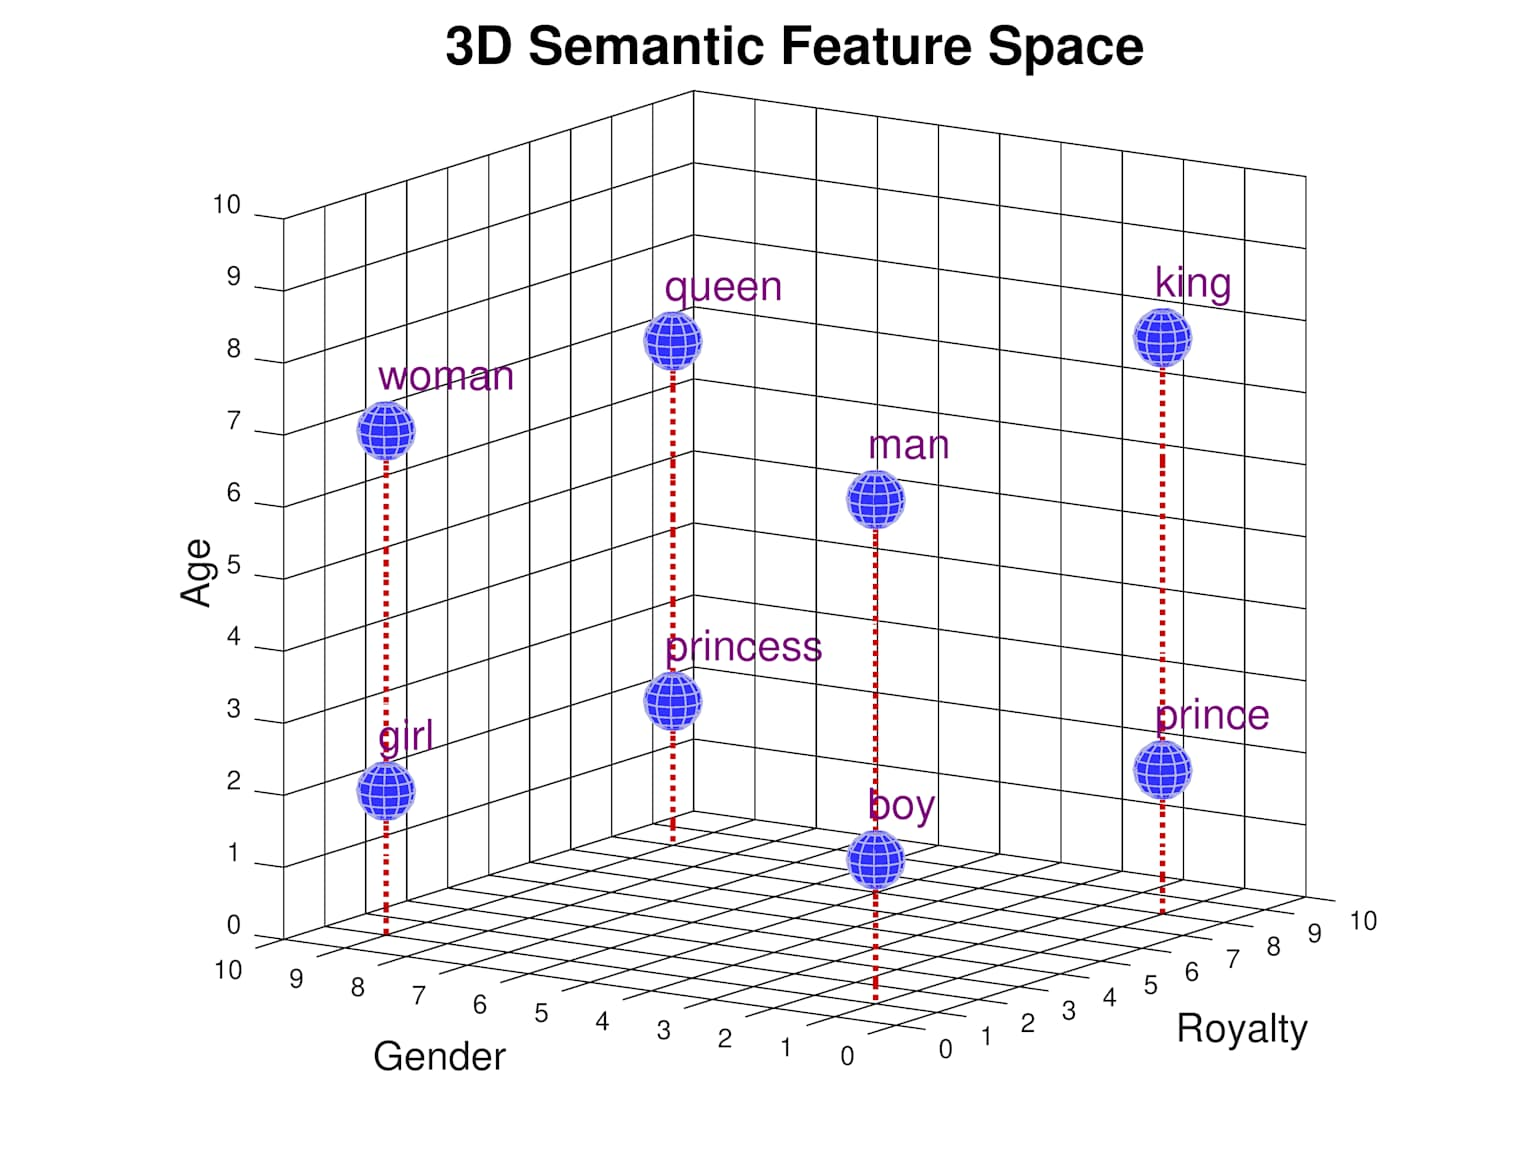
\includegraphics[width=0.85\textwidth]{5-Figures/Chapter2/king-queen-embedding}
    \caption{Word vector space learned by Word2Vec, illustrating semantic analogies such as $\vec{king} - \vec{man} + \vec{woman} \approx \vec{queen}$. Adapted from~\cite{mikolov2013word2vec}.}
    \label{fig:word2vec}
\end{figure}

By demonstrating that semantic similarity can be captured as geometric proximity
in a continuous vector space, Word2Vec turned the distributional hypothesis into
an actionable engineering principle. This insight directly underlies modern
embedding models and vector databases, central components of
Retrieval-Augmented Generation (RAG) pipelines~\cite{lewis2020rag}, and thus the
quality and cost of the embedding stage in the Maestro framework's RAG pipeline.

\subsection{The Transformer Architecture}
\label{sec:transformer}

Despite advances in distributed representations, sequence modelling remained
constrained by recurrent architectures such as LSTMs and GRUs, which process
tokens sequentially and suffer from vanishing gradients over long contexts.
Vaswani et al.~\cite{vaswani2017attention} proposed the Transformer, which
dispenses with recurrence entirely and relies solely on attention to model
dependencies between all positions in a sequence simultaneously. Its core
operation, scaled dot-product attention, computes outputs as a weighted sum of
value vectors, with weights derived from the compatibility between query and key
projections:

\[
\text{Attention}(Q, K, V) = \text{softmax}\!\left(\frac{QK^{T}}{\sqrt{d_k}}
\right)V
\]

\begin{figure}[htbp]
    \centering
    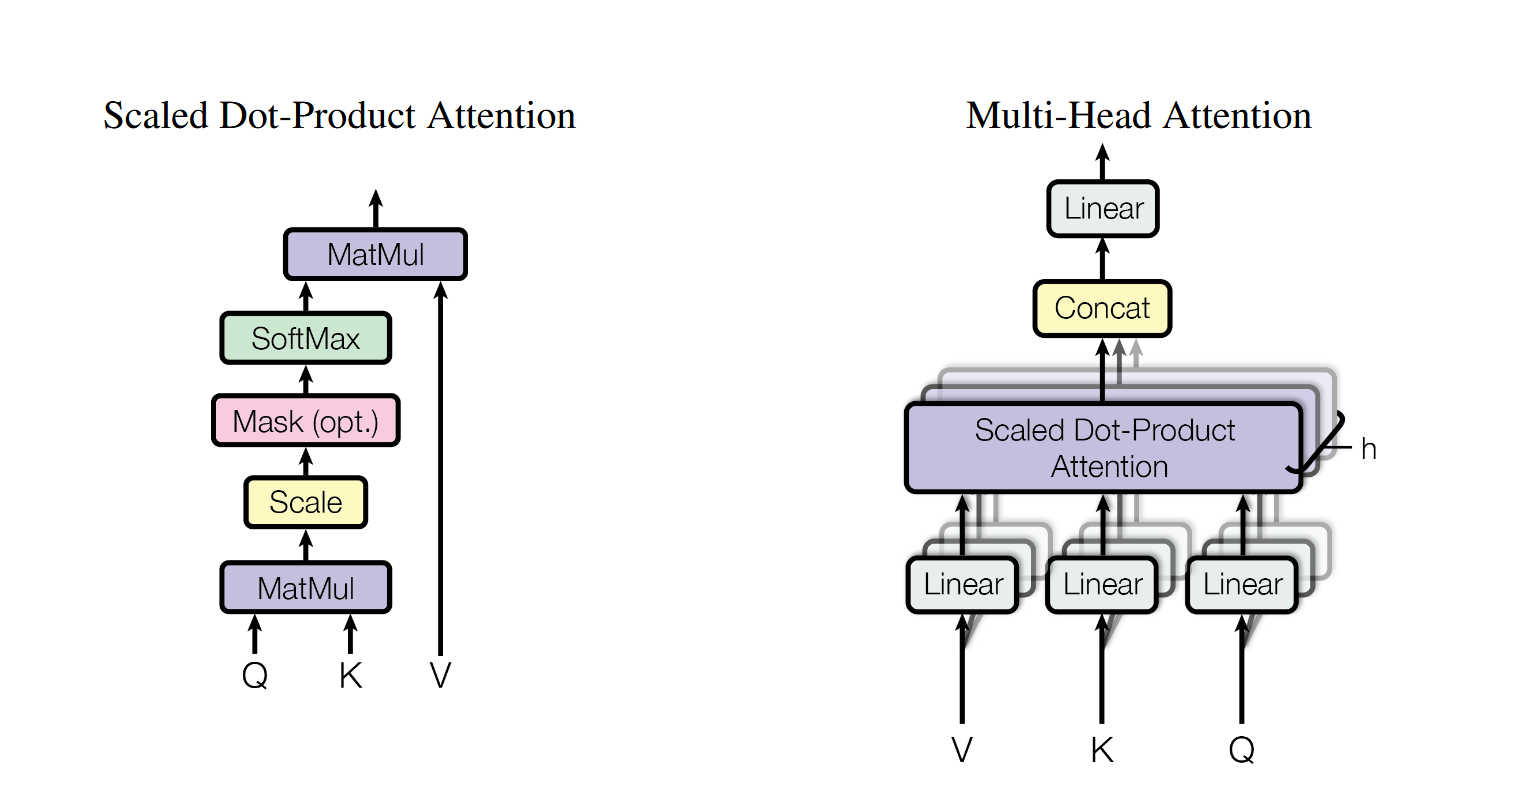
\includegraphics[width=0.85\textwidth]{5-Figures/Chapter2/scale-dot-multi-head}
    \caption{Scaled Dot-Product Attention (left) and Multi-Head Attention (right). Adapted from~\cite{vaswani2017attention}.}
    \label{fig:attention}
\end{figure}

By running several such operations in parallel - Multi-Head Attention - the
model attends simultaneously to different types of relationships, such as
syntactic dependencies and semantic co-references. Positional encodings are
added to the input embeddings to compensate for the architecture's permutation
invariance. The resulting model achieved 28.4 BLEU on the WMT 2014
English-to-German benchmark, surpassing all prior approaches at a fraction of
the training compute~\cite{vaswani2017attention}.

\begin{figure}[htbp]
    \centering
    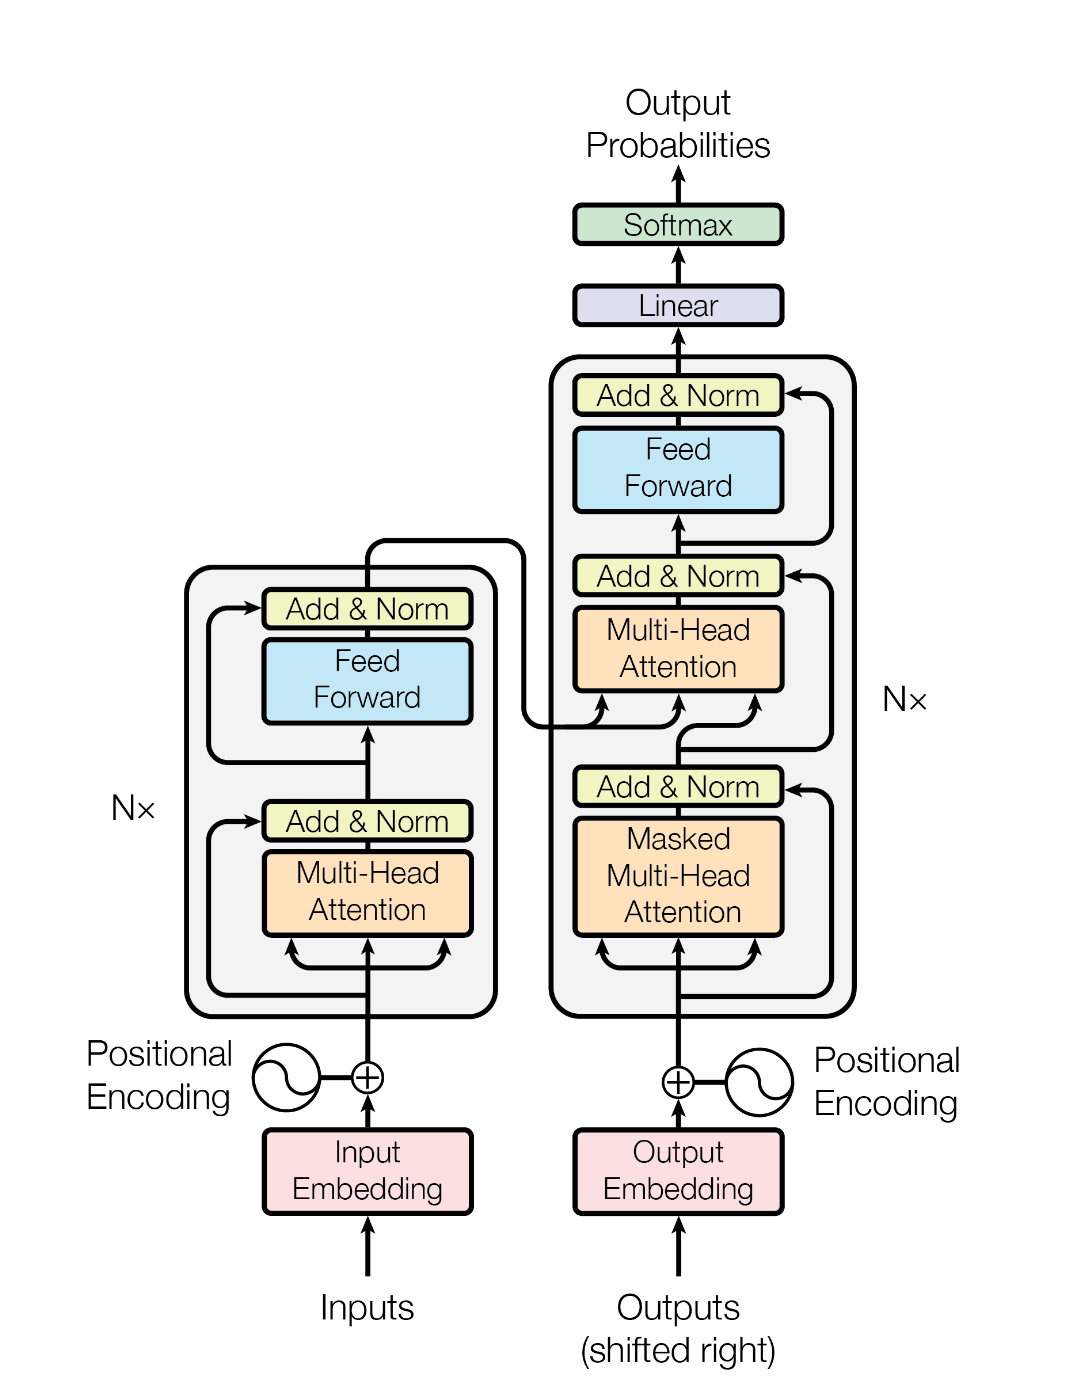
\includegraphics[width=0.50\textwidth]{5-Figures/Chapter2/transformer}
    \caption{Full Transformer architecture with encoder and decoder stacks. Adapted from~\cite{vaswani2017attention}.}
    \label{fig:transformer}
\end{figure}

The Transformer's parallelism over sequence positions unlocked a new scaling
regime. Derived architectures - encoder-only models such as
BERT~\cite{devlin2018bert} for representation learning, and decoder-only models
such as the GPT series~\cite{brown2020gpt3} for generation - became the standard
building blocks of enterprise GenAI systems. Critically, attention scales
quadratically with sequence length, \(O(n^2)\), making context length a primary
cost driver in token-priced LLM APIs. This property is foundational to the
FinOps strategies explored in this dissertation - prompt compression, semantic
caching, and dynamic model selection - each of which seeks to reduce the
effective \(n\) processed or the frequency of
inference~\cite{mikolov2013word2vec,vaswani2017attention}.

Together, these works define the representational substrate of modern GenAI:
Word2Vec encodes meaning as position in a learned vector space, and the
Transformer enables context-sensitive reasoning over such representations
efficiently and at scale. The remainder of this chapter examines the
architectural patterns, operational frameworks, and cost optimisation techniques
that build upon these foundations in production enterprise systems.

%%------------------------------------------------------------
%% SECTION: Large Language Models in Production
%% Covers: LLM overview and scaling laws, RLHF/instruction tuning,
%% open-weight models, and the enterprise deployment spectrum.
%%------------------------------------------------------------
\section{Large Language Models in Production}
\label{sec:llms-in-production}

Building upon distributed word representations and the Transformer, the field
consolidated around a unified paradigm - the large language model (LLM) - in
which ever-larger Transformer networks, pre-trained on internet-scale corpora,
acquire general-purpose competence that can be redirected to downstream tasks
with minimal additional supervision. This section characterizes LLMs as a class,
traces the evolution from raw pre-training to instruction-following alignment,
and examines the architectural and economic implications of deploying them at
enterprise scale.

\subsection{Large Language Models: An Overview}
\label{sec:llm-overview}

% Defines LLMs via the emergent-capability criterion; introduces decoder-only
% architecture and contrasts with encoder-only BERT; establishes scaling laws
% as the link between compute investment and token-cost motivation.
A large language model is a neural language model of sufficient parameter count
and training data scale that general linguistic and reasoning capabilities emerge
from the pre-training objective alone, without task-specific architectural
modification~\cite{brown2020gpt3}. Pre-training proceeds via self-supervised
next-token prediction over corpora of hundreds of billions to trillions of
tokens, yielding weights that encode an implicit representation of syntax,
semantics, world knowledge, and rudimentary reasoning chains, elicited through
natural language prompting.

LLMs are predominantly realized as \textit{decoder-only} Transformer
architectures~\cite{vaswani2017attention}, whose self-attention layers apply a
causal mask restricting each token's attention to its leftward context,
preserving autoregressive generation. This contrasts with the encoder-only
variant typified by BERT~\cite{devlin2018bert}, which produces bidirectional
representations for discriminative tasks. For generative applications, the
decoder-only paradigm dominates, and it is this class of model that underpins
the enterprise GenAI systems examined in this dissertation.

A defining empirical finding is the existence of \textit{scaling laws}:
power-law relationships between model size, training compute, dataset volume,
and downstream performance~\cite{brown2020gpt3}. Because performance is largely
predictable and improvable by increasing any of these axes, compute investment
translates into measurable capability gains. This has driven the successive
scaling of commercial models and made token consumption a dominant cost
variable - larger models process the same input more expensively - directly
motivating the cost optimization strategies central to this work.

\subsection{From Pre-training to Instruction Tuning}
\label{sec:instruction-tuning}

% Motivates the alignment gap between next-token pre-training and user intent;
% describes the three-stage RLHF pipeline (SFT → reward model → PPO) from
% InstructGPT; highlights the key empirical result that a 1.3B aligned model
% outperforms a 175B unaligned one - directly informing dynamic model selection.
Despite their generative competence, early LLMs exhibited systematic
misalignment between model behavior and user intent: a model trained only to
predict the next token continues text plausibly, but not necessarily in ways
that are \textit{helpful}, \textit{honest}, or \textit{harmless} when deployed
as an assistant. Ouyang et al.~\cite{ouyang2022instructgpt} addressed this gap
with a three-stage fine-tuning pipeline centered on Reinforcement Learning from
Human Feedback (RLHF).

First, a \textit{supervised fine-tuning} (SFT) phase trains the base model on
high-quality human demonstrations over a curated prompt distribution. Second, a
\textit{reward model} is trained to predict human preference scores over pairs
of outputs, internalizing a proxy for human judgment. Third, the SFT model is
optimized against this reward signal using Proximal Policy Optimization (PPO).
The resulting InstructGPT models, with as few as 1.3 billion parameters, were
consistently preferred by human evaluators over the unaligned 175-billion
parameter GPT-3 baseline, showing that alignment quality is not strictly a
function of scale~\cite{ouyang2022instructgpt}. This established RLHF as the
standard post-training procedure for production LLMs and confirmed that an
aligned smaller model can match or exceed a larger unaligned one - a
relationship that informs the dynamic model selection strategies explored in
this dissertation.

\subsection{Open-Weight Models and the Deployment Spectrum}
\label{sec:open-weight-models}

% Contrasts proprietary API models (GPT-4, Claude) with self-hostable
% open-weight alternatives (Llama 2); introduces the LLM cascading / dynamic
% model selection paradigm as the core cost-optimization mechanism evaluated
% in the Maestro framework.
The commercial LLM landscape is stratified between proprietary, API-accessed
models and openly released, self-hostable alternatives. The former, exemplified
by OpenAI's GPT-4 family and Anthropic's Claude series, exposes inference through
token-priced cloud APIs; the latter is represented most prominently by Meta AI's
Llama series. Touvron et al.~\cite{touvron2023llama2} introduced Llama~2, a
family of 7 to 70 billion parameter models pre-trained on two trillion tokens and
released for commercial use. RLHF-aligned variants (Llama~2-Chat) achieve
performance competitive with closed-source alternatives on standard benchmarks
while remaining locally deployable~\cite{touvron2023llama2}.

Capable open-weight models introduce a consequential degree of freedom into
enterprise GenAI architectures. Rather than committing to a single proprietary
provider, organizations may route inference dynamically across a portfolio of
models differentiated by capability tier, latency, and per-token cost. Smaller
open-weight models, deployed on-premise or on reserved instances, serve
high-volume, lower-complexity queries at reduced marginal cost, while frontier
API models handle tasks requiring peak reasoning. This routing paradigm -
\textit{LLM cascading} or \textit{dynamic model selection} - is a central cost
optimization mechanism evaluated in this dissertation in the context of the
Maestro framework's multi-cloud deployment~\cite{touvron2023llama2,
ouyang2022instructgpt}.

The progression from raw pre-training through RLHF alignment to the open-weight
deployment spectrum thus defines the operational environment for enterprise
GenAI frameworks. The ability to select, combine, and switch between models of
varying capability and cost is not merely an architectural convenience but a
financial imperative in production systems, where token consumption can scale
three to five times per client without deliberate
optimization~\cite{ouyang2022instructgpt}.

%%------------------------------------------------------------
%% SECTION: Retrieval-Augmented Generation
%% Covers: foundational RAG architecture (Lewis 2020), the Naive/Advanced/
%% Modular RAG taxonomy (Gao 2023), dense semantic retrieval with SBERT
%% (Reimers 2019), and the mapping onto LlamaIndex.
%%------------------------------------------------------------
\section{Retrieval-Augmented Generation}
\label{sec:rag}

Large language models store factual knowledge implicitly within their
parameters, which introduces well-documented limitations: parametric knowledge
is frozen at training time, cannot be transparently audited, and tends to
produce hallucinations when queries exceed the training
distribution~\cite{lewis2020rag}. Retrieval-Augmented Generation (RAG) addresses
these limitations by coupling a generative model with a dynamic, non-parametric
memory that can be queried, updated, and inspected at inference time. The
following subsections trace the theoretical foundations of the paradigm, its
architectural evolution, and the dense retrieval machinery that makes scalable
semantic search tractable.

% ------------------------------------------------------------
\subsection{Foundational Architecture: Lewis et al.\ (2020)}
\label{subsec:rag_foundation}

% Presents the two-component RAG model (DPR retriever + BART generator),
% the RAG-Sequence and RAG-Token marginalization strategies, and the
% hot-swappable non-parametric memory property relevant to production.
The canonical RAG formulation was introduced by Lewis et
al.~\cite{lewis2020rag}, who proposed a general-purpose fine-tuning recipe for
generative models endowed with an external non-parametric memory. The
architecture comprises two components: (i)~a \emph{retriever} $p_\eta(z \mid x)$,
implemented as a Dense Passage Retriever (DPR)~\cite{karpukhin2020dpr} whose
bi-encoder maps queries and documents into a shared dense vector space via
independent BERT encoders, and (ii)~a \emph{generator} $p_\theta(y_i \mid x, z,
y_{1:i-1})$, implemented as BART-large~\cite{lewis2020bart}, which conditions its
output on the concatenation of the query $x$ and retrieved passages $z$.

Formally, the top-$K$ passages are selected by solving a Maximum Inner Product
Search (MIPS) problem over a pre-indexed Wikipedia corpus of 21~million
100-word chunks:
%
\begin{equation}
    p_\eta(z \mid x) \;\propto\; \exp\!\left( d(z)^\top q(x) \right),
    \quad d(z) = \mathrm{BERT}_d(z),\; q(x) = \mathrm{BERT}_q(x).
\end{equation}
%
Two marginalization strategies over the latent document variable $z$ are
proposed. In \emph{RAG-Sequence}, a single retrieved document is assumed
responsible for the entire output sequence:
%
\begin{equation}
    p_{\mathrm{RAG\text{-}Seq}}(y \mid x)
    \;\approx\;
    \sum_{z \,\in\, \mathrm{top\text{-}}k}
    p_\eta(z \mid x)\;
    \prod_{i}^{N} p_\theta(y_i \mid x, z, y_{1:i-1}).
\end{equation}
%
In \emph{RAG-Token}, a distinct document may be selected at each generation step,
enabling the generator to synthesize content from multiple retrieved passages:
%
\begin{equation}
    p_{\mathrm{RAG\text{-}Token}}(y \mid x)
    \;\approx\;
    \prod_{i}^{N}
    \sum_{z \,\in\, \mathrm{top\text{-}}k}
    p_\eta(z \mid x)\;
    p_\theta(y_i \mid x, z, y_{1:i-1}).
\end{equation}
%
\begin{figure}[htbp]
    \centering
    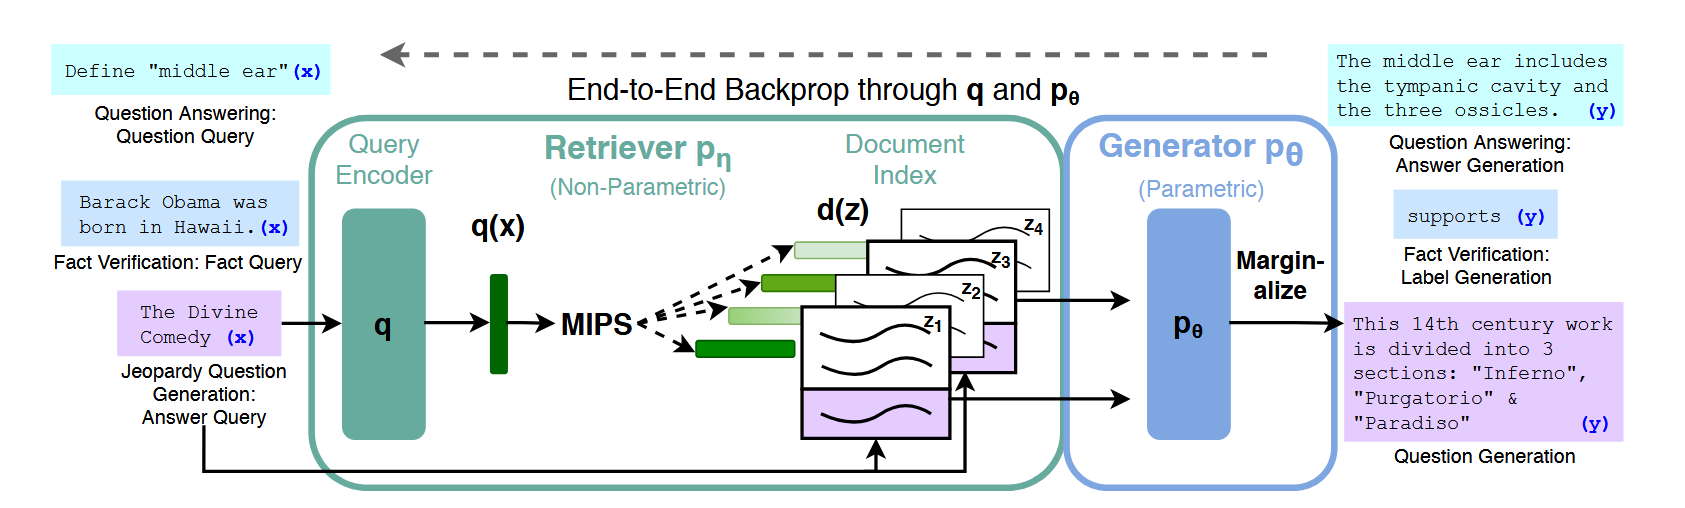
\includegraphics[width=0.85\textwidth]{5-Figures/Chapter2/rag-retriever-BART-MIPS}
    \caption{End-to-end RAG architecture combining a DPR retriever with a BART-large generator. Adapted from~\cite{lewis2020rag}.}
    \label{fig:rag-architecture}
\end{figure}

The retriever and generator are trained end-to-end by minimizing the negative
marginal log-likelihood $\sum_j -\log p(y_j \mid x_j)$, without direct
supervision on which documents to retrieve. The document encoder and its FAISS
index are frozen during fine-tuning; only the query encoder and BART generator
are updated, substantially reducing cost.

Empirically, RAG established state-of-the-art results on three open-domain
question answering benchmarks - Natural Questions (44.5 EM), WebQuestions (45.2
EM), and CuratedTrec (52.2 EM) - outperforming both parametric seq2seq baselines
(e.g.,\ T5-11B) and task-specific retrieve-and-extract systems~\cite{lewis2020rag}.
On Jeopardy question generation, human evaluators rated RAG outputs more factual
than BART in 42.7\% of trials versus 7.1\% favouring BART. An index-hotswapping
experiment further showed that replacing the document index updates the model's
world knowledge without retraining, a property of practical significance for
production deployments.

% ------------------------------------------------------------
\subsection{Architectural Evolution: Naive, Advanced, and Modular RAG}
\label{subsec:rag_survey}

% Applies the three-tier taxonomy of Gao et al. (2023): Naive RAG failure modes,
% Advanced RAG pre/post-retrieval interventions, and Modular RAG composable
% pipelines (ITER-RETGEN, FLARE, Self-RAG). Establishes RAG vs. fine-tuning tradeoff.
Gao et al.~\cite{gao2023ragsurvey} systematize the rapid evolution of RAG methods into a
three-tier taxonomy, providing a structural lens through which the design of
contemporary systems can be evaluated.

\begin{figure}[htbp]
    \centering
    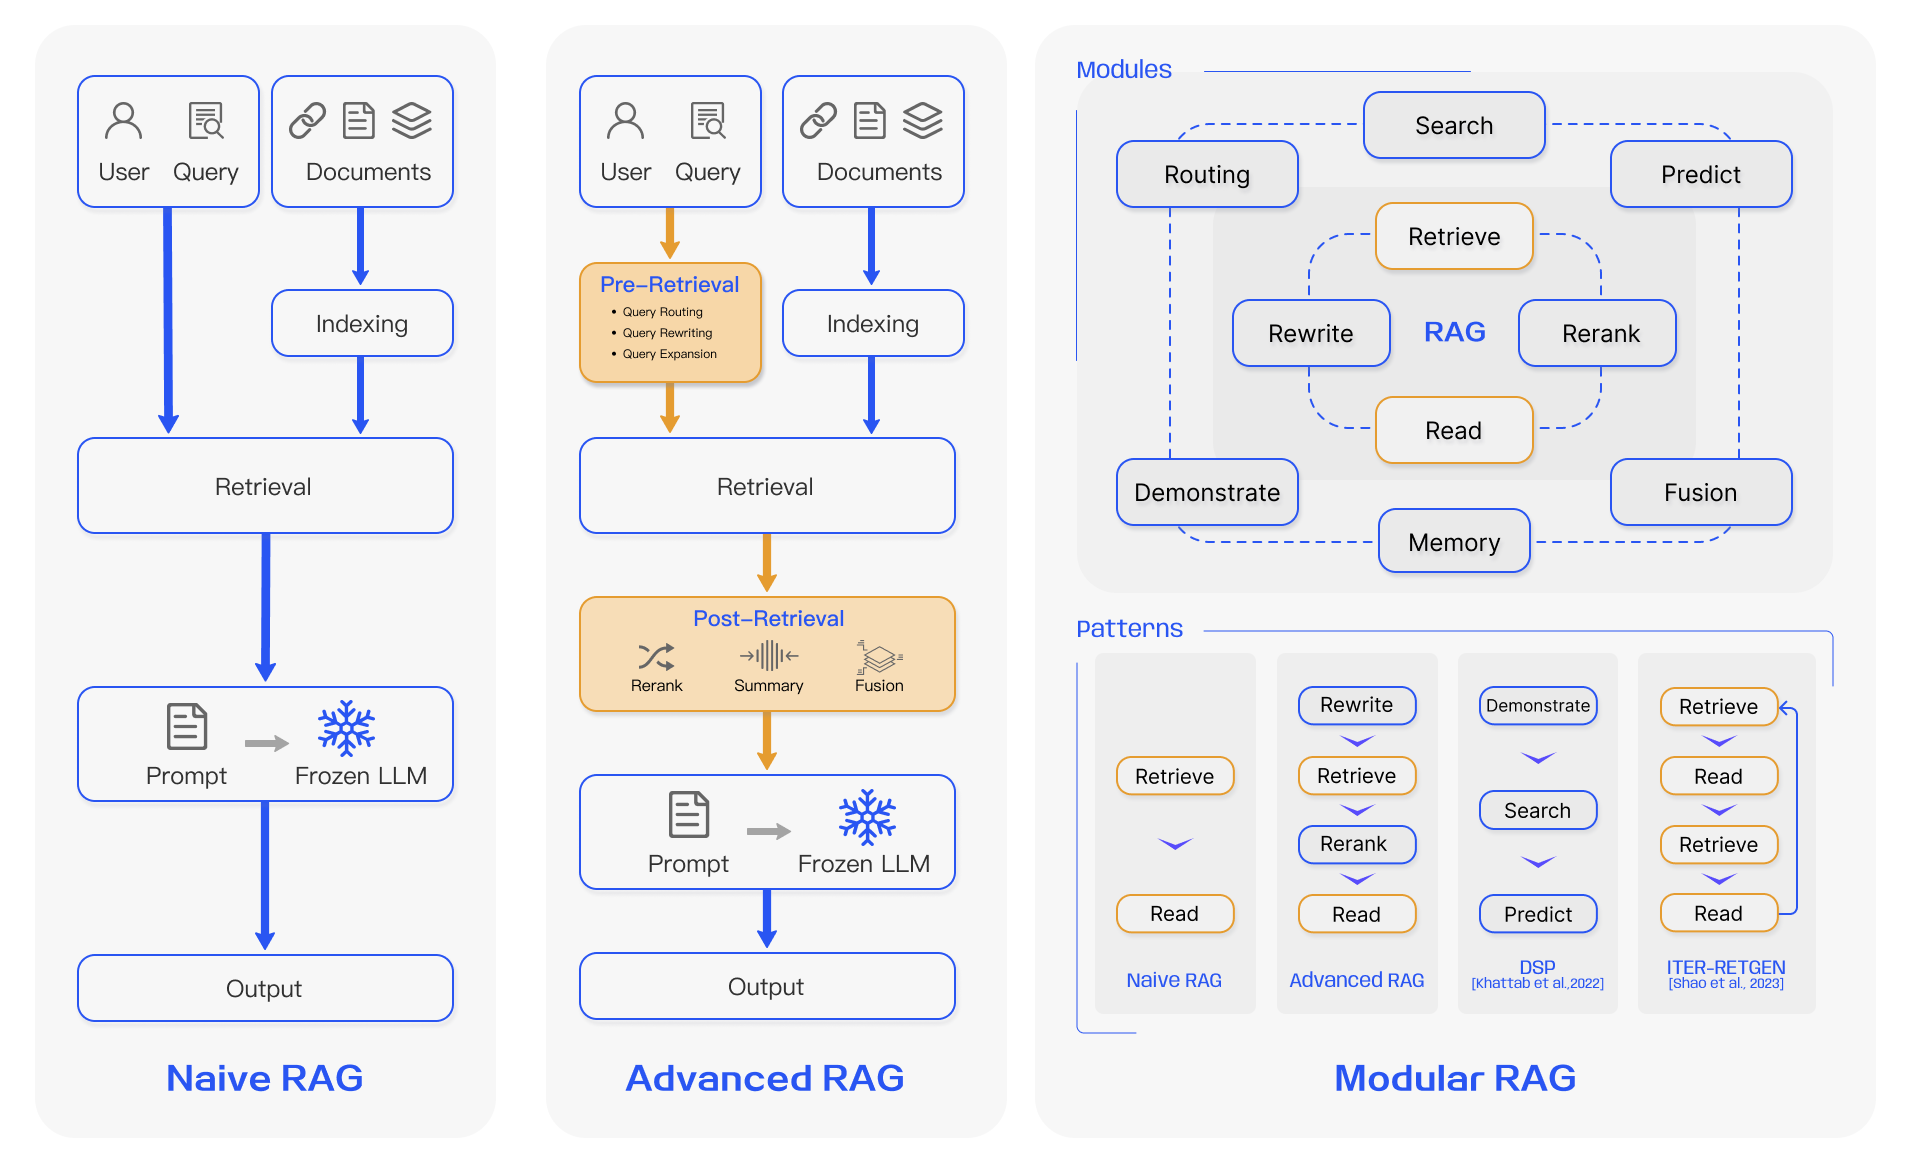
\includegraphics[width=0.85\textwidth]{5-Figures/Chapter2/naive-advanced-modular}
    \caption{Three-tier RAG taxonomy: Naive, Advanced, and Modular RAG. Adapted from~\cite{gao2023ragsurvey}.}
    \label{fig:rag-taxonomy}
\end{figure}

\paragraph{Naive RAG.}
The earliest post-ChatGPT implementations follow a minimal
\emph{Retrieve-then-Read} pipeline of three steps: (1)~\emph{indexing}, where
documents are chunked, encoded, and stored in a vector database;
(2)~\emph{retrieval}, where the top-$K$ chunks most similar to the query are
identified via cosine similarity; and (3)~\emph{generation}, where the query and
retrieved chunks form a prompt for the language model~\cite{gao2023ragsurvey}.
While effective in simple scenarios, Naive RAG exhibits well-characterized
failure modes: low retrieval precision from semantic gaps, context-window
saturation from uninformative passages, and hallucinations when the generator
defaults to parametric knowledge amid noisy context.

\paragraph{Advanced RAG.}
Advanced RAG introduces targeted pre- and post-retrieval interventions to
address the precision and coherence limitations of the naive
approach~\cite{gao2023ragsurvey}. Pre-retrieval strategies include query
rewriting, query expansion into sub-questions, and \emph{Hypothetical Document
Embeddings} (HyDE), where the model generates a hypothetical answer whose
embedding retrieves semantically closer passages. Post-retrieval strategies
include cross-encoder reranking and context compression to eliminate redundant
content before generation. Indexing enhancements - sliding-window chunking,
fine-grained segmentation, and metadata attachment - further improve recall and
temporal awareness. These modifications retain the linear Retrieve-then-Read
structure while substantially improving generation quality.

\paragraph{Modular RAG.}
Modular RAG supersedes the fixed pipeline by decomposing the system into
composable functional modules: \emph{Search}, \emph{Memory}, \emph{Routing},
\emph{Predict}, and \emph{Task Adapter}~\cite{gao2023ragsurvey}. This supports
non-sequential execution, including iterative retrieval loops (e.g.,\
ITER-RETGEN~\cite{shao2023iterretgen}), adaptive retrieval triggered by
generation uncertainty (e.g.,\ FLARE~\cite{jiang2023flare}), and self-reflective
retrieval (e.g.,\ Self-RAG~\cite{asai2023selfrag}). The design also enables
integration with complementary techniques - fine-tuning the retriever, the
generator, or both - without architectural changes. Gao et
al.~\cite{gao2023ragsurvey} position Modular RAG as the current frontier, whose
flexibility allows orchestration patterns that static pipelines cannot
accommodate.

A practical implication is that RAG and fine-tuning are not mutually exclusive.
RAG excels where knowledge must be updated frequently and interpretable
provenance is required, whereas fine-tuning suits stylistic adaptation or the
internalization of domain-specific reasoning. In knowledge-intensive tasks, Gao
et al.~\cite{gao2023ragsurvey} report that RAG consistently outperforms
unsupervised fine-tuning, on both pre-training knowledge and novel facts.

% ------------------------------------------------------------
\subsection{Dense Semantic Retrieval: Sentence-BERT}
\label{subsec:sbert}

% Motivates SBERT over vanilla BERT for large-scale semantic search
% (O(n^2) → O(1) lookup); describes Siamese/triplet architecture and the
% three training objectives; connects to embedding models used in RAG pipelines.
The retrieval component of a RAG pipeline depends critically on the quality and
tractability of sentence-level embeddings. Vanilla BERT is unsuitable for
large-scale semantic search: because it processes sentence pairs jointly through
a cross-attention encoder, finding the most similar pair among $n$~sentences
requires $\mathcal{O}(n^2)$ inference passes - approximately 65~hours for $n =
10{,}000$~\cite{reimers2019sbert}. Moreover, averaging BERT token embeddings or
using the \texttt{[CLS]} output yields representations that underperform even
GloVe on semantic textual similarity (STS) tasks, owing to BERT's lack of
explicit metric learning for sentence geometry.

Reimers and Gurevych~\cite{reimers2019sbert} address this by introducing
\emph{Sentence-BERT} (SBERT), a modification using Siamese and triplet network
structures to produce fixed-size, semantically meaningful sentence embeddings
amenable to efficient cosine-similarity comparison.

\begin{figure}[htbp]
    \centering
    \begin{minipage}[t]{0.48\textwidth}
        \centering
        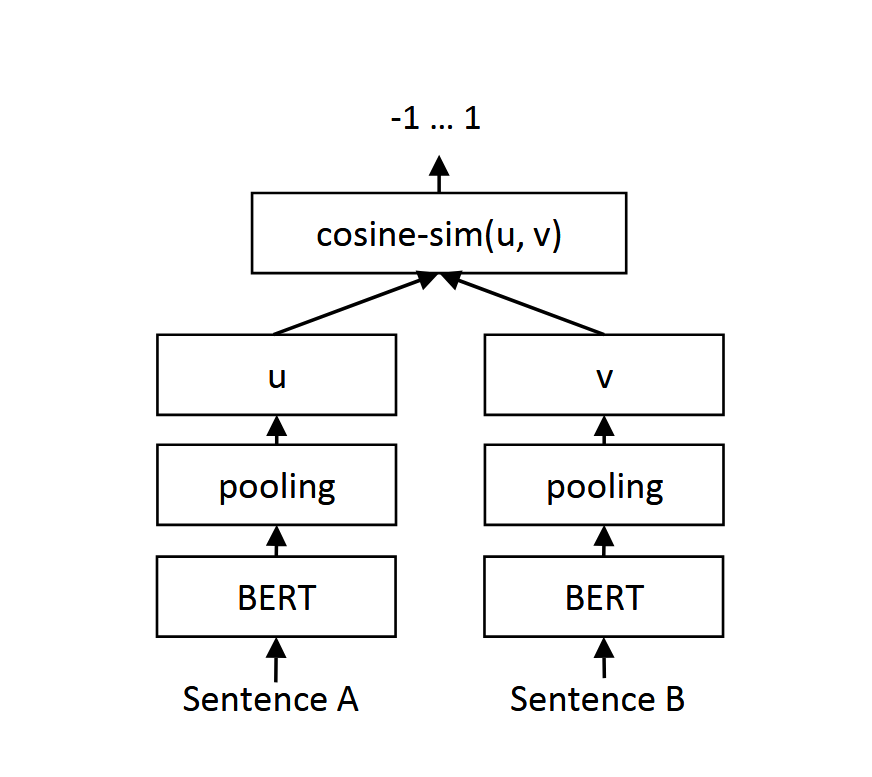
\includegraphics[width=\textwidth]{5-Figures/Chapter2/sbert-network-anchor-positive-negative}
        \label{fig:sbert-triplet}
    \end{minipage}\hfill
    \begin{minipage}[t]{0.48\textwidth}
        \centering
        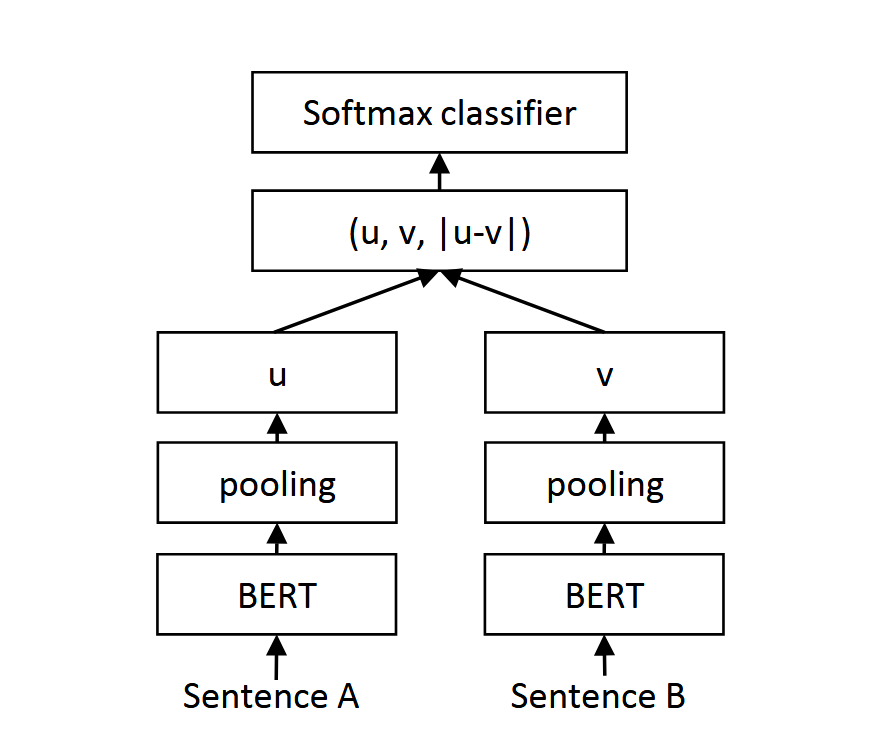
\includegraphics[width=\textwidth]{5-Figures/Chapter2/sbert-class-regress}
        \label{fig:sbert-objectives}
    \end{minipage}
    \caption{
        (Left) SBERT Siamese network architecture with triplet loss objective.
        (Right) Classification and regression training objectives of SBERT.
        Adapted from~\cite{reimers2019sbert}.
    }
\end{figure}

The architecture passes each sentence independently through a shared BERT
encoder, then mean-pools the output token embeddings into single vectors
$\mathbf{u}$ and $\mathbf{v}$ for a sentence pair. Three training objectives are
supported, depending on the available supervision:
%
\begin{itemize}
    \item \textbf{Classification objective} (for NLI corpora): a softmax
    classifier over the concatenation $[\mathbf{u};\, \mathbf{v};\,
    |\mathbf{u} - \mathbf{v}|]$ trained to predict entailment, contradiction, or
    neutral labels.
    \item \textbf{Regression objective} (for STS corpora): cosine-similarity
    between $\mathbf{u}$ and $\mathbf{v}$ optimized with mean-squared error
    against human-annotated similarity scores.

    \item \textbf{Triplet objective}: a margin-based ranking loss that ensures the
    anchor embedding $\mathbf{a}$ is closer to a positive $\mathbf{p}$ than to a
    negative $\mathbf{n}$ by a margin $\epsilon$:
    %
    \begin{equation}
        \mathcal{L}_{\mathrm{triplet}}
        = \max\!\left(
            \|\mathbf{a} - \mathbf{p}\| - \|\mathbf{a} - \mathbf{n}\| + \epsilon,\;0
          \right).
    \end{equation}
\end{itemize}
%
The Siamese design decouples encoding from comparison: document embeddings are
computed once at indexing time, reducing query-time inference to a single forward
pass plus a nearest-neighbor lookup. This cuts the 65-hour pairwise comparison to
roughly 5 seconds for a 10,000-sentence corpus, while preserving or improving
BERT's STS accuracy~\cite{reimers2019sbert}: SBERT gains 11~Spearman points over
InferSent and 5~over Universal Sentence Encoder.

% ------------------------------------------------------------
\subsection{Connection to LlamaIndex}
\label{subsec:rag_llamaindex}

% Maps the theoretical RAG contributions above onto LlamaIndex abstractions:
% ingestion → SentenceSplitter, embedding → SBERT-compatible models,
% retrieval → VectorStoreIndex MIPS, advanced patterns → RouterQueryEngine
% and ReActAgent. Positions LlamaIndex as a production-grade Modular RAG system.
The contributions reviewed above map directly onto LlamaIndex, the framework
employed in this work. LlamaIndex operationalizes the RAG pipeline of Lewis et
al.~\cite{lewis2020rag} through a modular architecture separating ingestion,
indexing, retrieval, and synthesis~\cite{liu2022llamaindex}. During
\emph{ingestion}, \texttt{SimpleDirectoryReader} loads documents that
\texttt{SentenceSplitter} segments into overlapping chunks - a direct
implementation of the Advanced RAG chunking strategies of Gao et
al.~\cite{gao2023ragsurvey}. The resulting nodes are encoded via a configurable
embedding model (\texttt{Settings.embed\_model}), defaulting to OpenAI's
\texttt{text-embedding-3-small} but readily replaced by any SBERT-compatible
HuggingFace model (e.g.,\ \texttt{BAAI/bge-small-en-v1.5}), whose architecture
descends from the Siamese paradigm of Reimers and
Gurevych~\cite{reimers2019sbert}.

At query time, \texttt{VectorStoreIndex} retrieves the top-$K$ nodes via cosine
similarity - the same MIPS formulation as DPR in~\cite{lewis2020rag} - and passes
them with the query to the language model for synthesis. The framework further
exposes advanced patterns consistent with the Modular RAG taxonomy of Gao et
al.~\cite{gao2023ragsurvey}: \texttt{RouterQueryEngine} routes semantically to
sub-indexes; reranking modules (e.g.,\ \texttt{SentenceTransformerRerank}) apply
cross-encoder scoring; and iterative retrieval agents can be composed from
\texttt{ReActAgent}. LlamaIndex thus provides a production-grade instantiation of
the entire RAG design space surveyed by Gao et al.~\cite{gao2023ragsurvey},
grounded in the dense retrieval foundations of Lewis et al.~\cite{lewis2020rag}
and Reimers and Gurevych~\cite{reimers2019sbert}.

%%------------------------------------------------------------
%% SECTION: Frameworks, MCP and Maestro
%%------------------------------------------------------------
\section{Frameworks, MCP and Maestro}
\label{sec:orchestration}

The preceding sections - dense vector representations, attention-based language
models, retrieval-augmented generation, and dense semantic retrieval - describe
the \emph{components} of a modern GenAI system, but not how they are composed,
governed, and operated at production scale. This section addresses that gap
across three layers of increasing practical specificity.

\subsection{LLM Orchestration Frameworks}
\label{sec:orchestration-frameworks}

The emergence of capable LLMs created an immediate engineering challenge:
composing LLMs with external tools, persistent memory, and retrieval systems into
coherent, repeatable pipelines. LangChain~\cite{chase2022langchain} addressed
this with three core primitives. A \textit{chain} is a composable sequence of
calls - to an LLM, retriever, tool, or another chain - assembled declaratively
and reused across applications. A \textit{tool} is any callable capability
exposed with a name, a natural-language description, and a typed input schema,
which the LLM uses to decide at runtime which tool to invoke and with what
arguments. \textit{Memory} modules attach conversational context to a chain,
enabling stateful multi-turn interactions. Together these define the dominant
orchestration pattern in the field: a model-centric loop in which the LLM selects
and sequences external capabilities.

The theoretical foundation for this loop was established by
\cite{yao2022react}~\cite{yao2022react}, who proposed the \textsc{ReAct}
paradigm (\textit{Reason + Act}). Rather than separating chain-of-thought
reasoning from tool use, \textsc{ReAct} interleaves them in a single iterative
cycle: the model emits a \textit{Thought}, selects an \textit{Action} (a tool
call), receives an \textit{Observation} (the tool output), and repeats until a
terminal condition is met. On multi-step knowledge-intensive tasks - HotpotQA,
FEVER, ALFWorld, and WebShop - \textsc{ReAct} outperformed both chain-of-thought
and action-only baselines, showing that tight coupling of reasoning and acting is
essential for robust agent behavior~\cite{yao2022react}. This loop is the
intellectual ancestor of every subsequent agent executor, including LangChain's
\texttt{AgentExecutor}, and it directly informs the orchestration design of the
system examined in this work.

\begin{figure}[htbp]
    \centering
    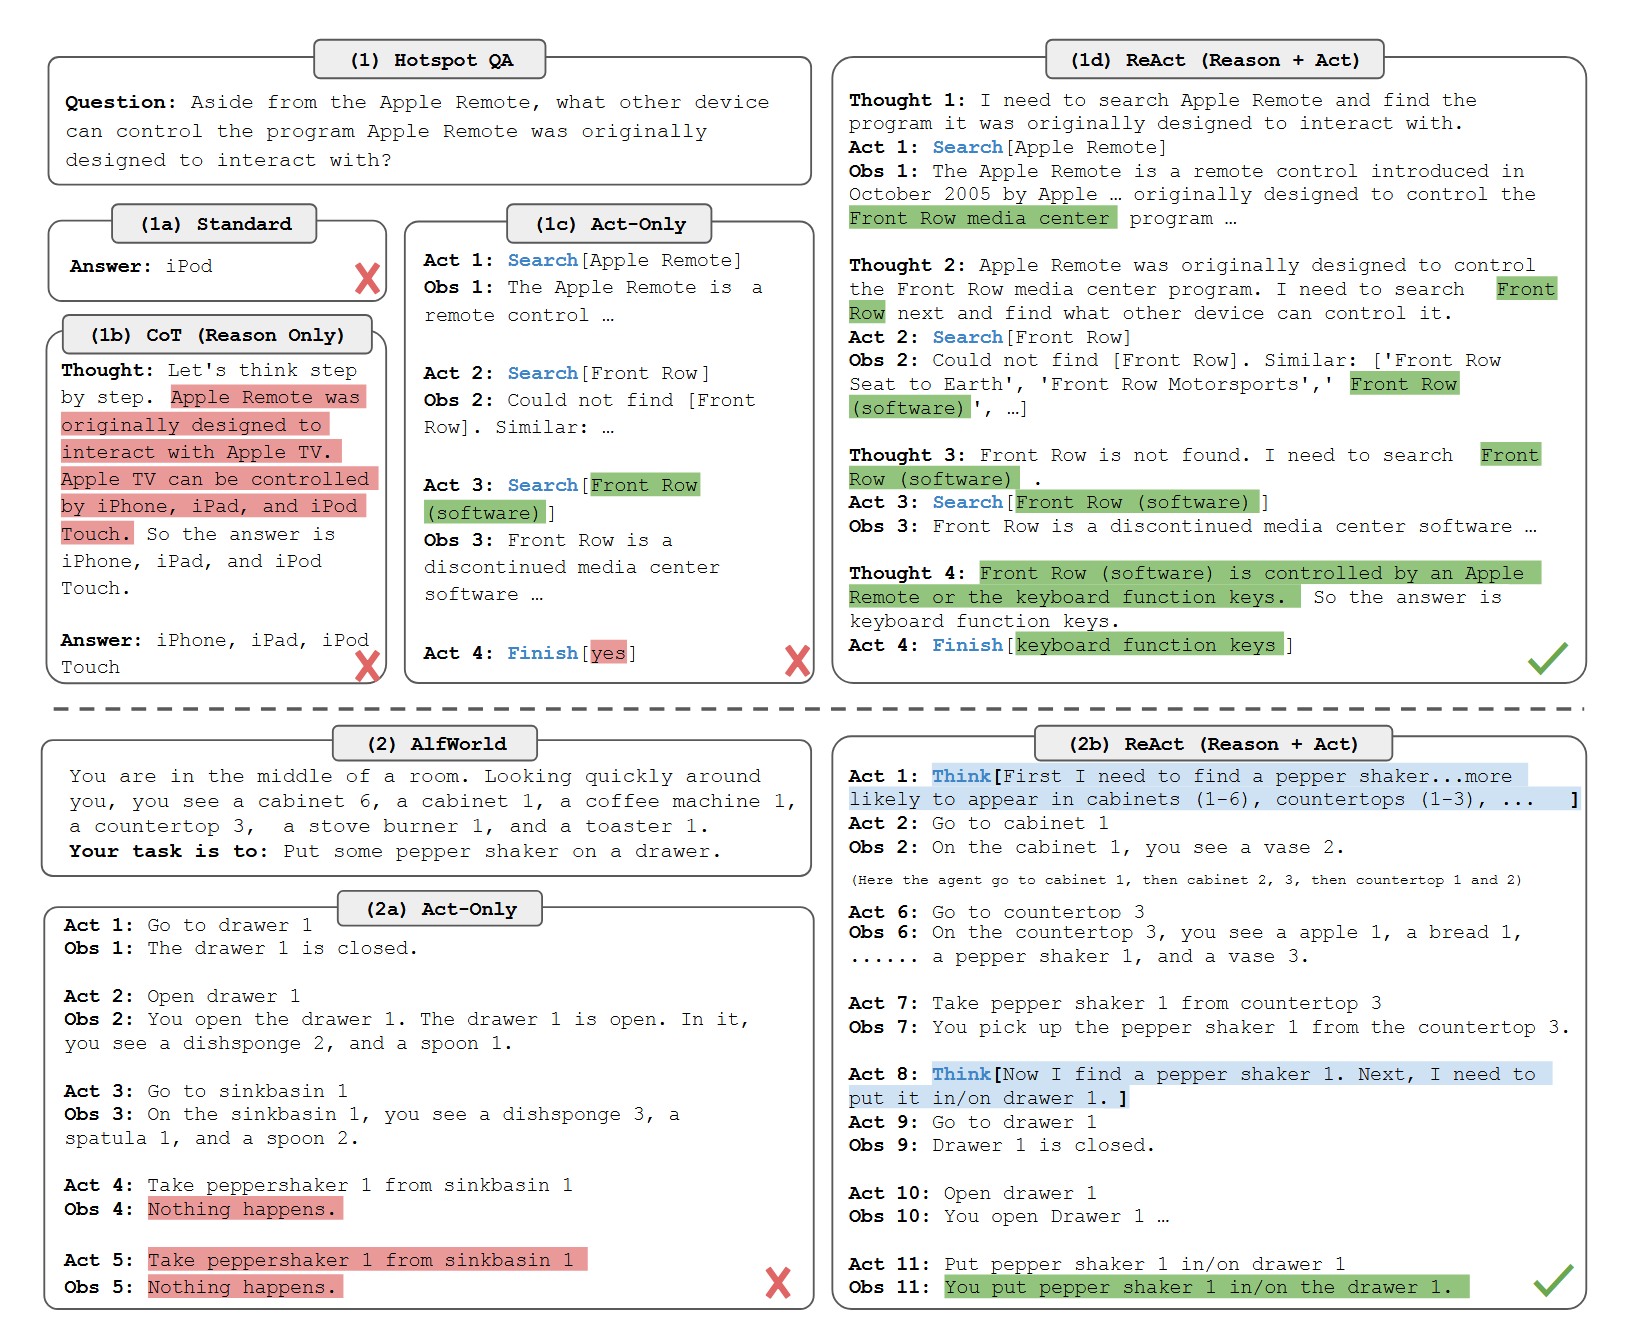
\includegraphics[width=0.85\textwidth]{5-Figures/Chapter2/reAct-loop}
    \caption{The \textsc{ReAct} reasoning loop interleaving \textit{Thought},
    \textit{Action}, and \textit{Observation} steps. Adapted from~\cite{yao2022react}.}
    \label{fig:react-loop}
\end{figure} 

\subsection{Model Context Protocol}
\label{sec:mcp}

A persistent weakness of this orchestration paradigm is the absence of a standard
interface between agents and the systems they invoke. Each integration is
bespoke: a tool written for LangChain is not directly consumable by another
framework, and a function registered for OpenAI's function-calling API is
invisible to a Claude-based agent. This $N \times M$ integration problem - $N$
agent frameworks times $M$ external services - generates duplicated adapter code,
inconsistent error handling, and fragile dependency chains that impede
development velocity and maintainability~\cite{anthropic2024mcp}.

\begin{figure}[htbp]
    \centering
    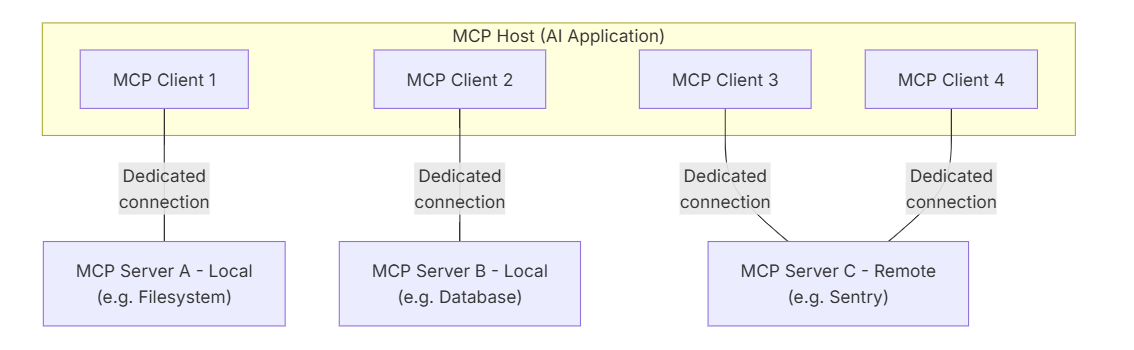
\includegraphics[width=0.85\textwidth]{5-Figures/Chapter2/mcp-architecture}
    \caption{Model Context Protocol architecture showing the Host, Client, and Server roles connected via JSON-RPC~2.0. Adapted from~\cite{modelcontextprotocol2024}.}
    \label{fig:mcp-architecture}
\end{figure}

The Model Context Protocol (MCP), introduced by Anthropic in
2024~\cite{anthropic2024mcp} and fully specified in its reference
documentation~\cite{modelcontextprotocol2024}, addresses this with an open,
transport-agnostic protocol standardizing how LLM hosts expose and consume
external capabilities. It defines three roles. An \textit{MCP Host} is the
application embedding the LLM - a development environment, chat interface, or
agent runtime. An \textit{MCP Client} manages the host's connections to servers.
An \textit{MCP Server} is a lightweight process exposing a bounded set of
capabilities over JSON-RPC~2.0, via either standard I/O (local) or HTTP with
Server-Sent Events (remote)~\cite{modelcontextprotocol2024}. Capabilities are
organized into three primitives: \textit{Tools} (functions invoked with
structured arguments, analogous to LangChain tools but protocol-defined),
\textit{Resources} (read-only data artifacts such as file contents, database
schemas, or live API responses), and \textit{Prompts} (parameterized templates
offered for reuse)~\cite{anthropic2024mcp, modelcontextprotocol2024}.

The distinction from vendor-specific function calling is substantive. OpenAI's
mechanism is stateless, scoped to a single provider, and leaves serialization,
discovery, and transport to the host. MCP is stateful, provider-agnostic, and
supports dynamic capability discovery: a client can query any server for its
current tool and resource catalog without prior knowledge of its implementation.
This reduces the integration surface from $N \times M$ to $N + M$ - any compliant
host interoperates with any compliant server, regardless of the LLM or framework.
This interoperability is directly relevant to multi-cloud enterprise deployments,
where exposing heterogeneous data services across Azure, AWS, and GCP through a
single protocol layer has significant governance and maintainability
implications.

\subsection{Enterprise GenAI Frameworks: Maestro in Context}
\label{sec:maestro}

Research prototypes built on LangChain and paradigms such as \textsc{ReAct}
operate under assumptions that enterprise production environments do not share.
For a deployment serving multiple tenants, correctness and capability are
necessary but insufficient: the system must also satisfy identity-based access
control, secret management, encryption at rest and in transit, token- and
model-level cost observability, multi-tenancy isolation, cross-provider
portability, and reliability under variable load - none of which are first-class
concerns in the orchestration literature above. Meeting these demands an
architectural discipline beyond assembling chains and tools: a governed platform
in which each component is independently deployable, swappable without contract
changes, and instrumented for both monitoring and audit compliance.

The Maestro GenAI Framework, developed by Closer Consulting, is a practitioner
response to precisely this gap~\cite{closer2025maestro}. Validated across
production deployments in the energy, healthcare, financial, and pharmaceutical
sectors, Maestro is a multi-repository, container-native microservices platform
that decomposes the RAG pipeline into independently governed services. The
\textit{LLM microservice} is a provider-agnostic gateway routing generation
requests to Azure OpenAI (GPT-4o, GPT-4o-mini), OpenAI, Azure AI Services
(Mistral-Nemo, DeepSeek-R1), and Google Gemini behind a stable contract. The
\textit{orchestrator} (chatbot-backend) implements the \textsc{ReAct}-derived RAG
loop - history retrieval, hybrid vector search, per-chunk relevance filtering,
prompt assembly, and LLM invocation - as a FastAPI service backed by LangChain.
The \textit{vector database service} handles ingestion, chunking, embedding via
\texttt{text-embedding-ada-002}, and hybrid kNN+BM25 retrieval over MongoDB
Atlas. The \textit{datastore microservice} provides a provider-agnostic
persistence layer over Azure Cosmos~DB and MongoDB for chat history, feedback,
and document metadata. A \textit{guardrails microservice} performs PII detection
via Microsoft Presidio for Portuguese inputs. Two \textit{frontend surfaces} - a
Streamlit chatbot with Microsoft Entra~ID authentication and an Angular
back-office for prompt and question management - complete the user-facing layer.
Infrastructure is managed via OpenTofu targeting Azure, with observability through
OpenTelemetry and Azure Monitor. In production, the framework has demonstrated
measurable impact: one deployment serving over~600 daily active users with 4,000
daily interactions across five LLM models, and another achieving 83\%
question-answering accuracy over 2,907 indexed legal
documents~\cite{closer2025maestro}.

\begin{figure}[htbp]
    \centering
    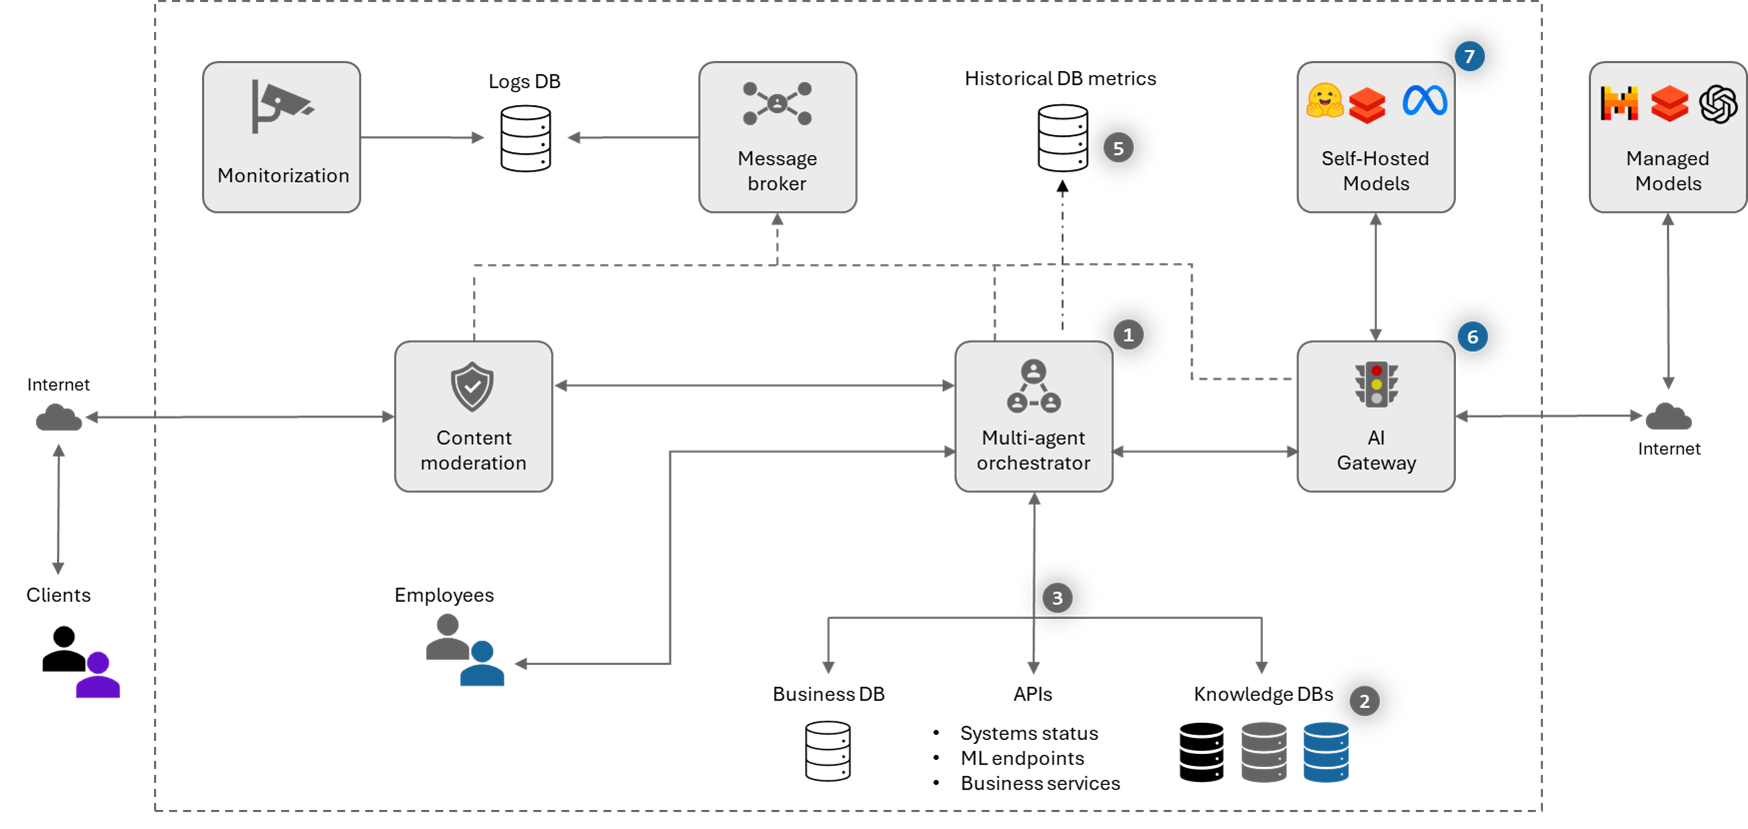
\includegraphics[width=0.85\textwidth]{5-Figures/Chapter2/maestro-architecture}
    \caption{Functional architecture of the Maestro GenAI Framework, illustrating the \textit{multi-agent orchestrator}, \textit{AI Gateway}, \textit{content moderation}, self-hosted and managed model endpoints, and observability layer. Adapted from~\cite{closer2025maestro}.}
    \label{fig:maestro-functional}
\end{figure}

Despite this maturity, a systematic analysis of the current implementation
reveals structural limitations along three dimensions: the absence of a
standardized tool-exposure protocol - each microservice is reachable only through
bespoke REST endpoints, with no dynamic capability discovery or external
interoperability; an incomplete cost-observability and optimization layer - token
usage and per-model cost are not exported as metrics, and no semantic caching or
routing reduces redundant invocations; and an orchestration architecture relying
on hand-crafted orchestrators rather than a composable, reusable agent graph.
These three dimensions constitute the research frontier
% TODO: Placeholder cross-refs - replace when real sections exist:
%   - add \label{sec:maestro-mcp-extension} / \label{sec:maestro-orchestration-evolution}, or
%   - rephrase to Chapters~\ref{cha:design}--\ref{cha:implementation} (or other final structure).
addressed in Section~\ref{sec:maestro-mcp-extension}--\ref{sec:maestro-orchestration-evolution} of
this work.%
\todo[inline]{%
\textbf{[TODO]} Section range above uses placeholder labels; update references when those sections are written.%
}

%%------------------------------------------------------------
%% SECTION: Multi-Cloud Computing and Infrastructure as Code
%% Covers: foundational properties of cloud computing (Armbrust 2010),
%% interoperability and portability (Petcu 2013), IaC research landscape
%% (Rahman et al. 2019), and OpenTofu in Maestro (closer2025maestro).
%%------------------------------------------------------------
\section{Multi-Cloud Computing and Infrastructure as Code}
\label{sec:multi-cloud}

Deploying production-grade GenAI systems at enterprise scale is not a purely
algorithmic challenge but equally an infrastructural one. The components surveyed
above - LLMs, RAG pipelines, embedding models, and orchestration frameworks -
must ultimately be provisioned, networked, secured, and operated on physical or
virtual compute. Choices at this layer directly influence cost, resilience, and
vendor dependency, each a first-class design concern in Maestro. This section
examines the foundations of cloud computing and multi-cloud strategy, the
interoperability and portability challenges of heterogeneous deployments, the
research landscape of Infrastructure as Code, and the role of declarative
provisioning in making reproducible, provider-agnostic infrastructure management
tractable at scale.

%%------------------------------------------------------------
\subsection{Foundations of Cloud Computing}
\label{subsec:cloud-foundations}

\cite{armbrust2010view} identified three properties that distinguish cloud
computing from prior infrastructure paradigms: the \emph{illusion of infinite
resources} on demand, the \emph{elimination of upfront capital commitments}, and
the ability to \emph{pay for resources short-term} and release them when no
longer needed. Together these enable a shift from capital expenditure (CapEx),
where organizations maintain underutilized on-premises hardware, to operational
expenditure (OpEx), where compute cost tracks actual consumption. Armbrust et
al.\ showed that average server utilization in traditional data centers is only
5--20\%, whereas elastic provisioning lets organizations track real demand. This
matters for AI-intensive workloads, whose inference load is bursty and hard to
predict: on-demand provisioning without upfront commitment is precisely what
makes multi-model, multi-provider GenAI deployments economically viable.

The same work identified persistent obstacles to cloud adoption, two of which are
relevant here. \emph{Data lock-in} arises when data and application state become
tightly coupled to a single provider's proprietary formats, making migration
costly and creating asymmetric negotiating power. \emph{Service availability}
concerns the concentration of operational risk in one provider, where outages or
unilateral policy changes propagate to all dependent workloads. Armbrust et al.\
identified distributing workloads across independent providers as the principal
mitigation for both~\cite{armbrust2010view}. This is the foundational rationale
for multi-cloud architectures and anticipates Maestro's design philosophy, which
provisions compute and inference capacity across Azure, AWS, and GCP rather than
committing to any single platform~\cite{closer2025maestro}.

%%------------------------------------------------------------
\subsection{Interoperability and Portability in Multi-Cloud Environments}
\label{subsec:multi-cloud-interop}

Deploying applications across heterogeneous providers introduces engineering
challenges that replication alone does not resolve. Pectu~\cite{petcu2013interoperability}
formalized these by distinguishing two concerns: \emph{portability}, the capacity
to transfer a workload between cloud environments with bounded effort, and
\emph{interoperability}, the capacity for components on different clouds to
communicate at runtime. Both require explicit architectural investment and
neither emerges spontaneously from layering services across providers.

Petcu identified four sources of lock-in: proprietary APIs exposing non-standard
resource abstractions; divergent data formats impeding cross-provider movement;
incompatible service-level agreements preventing unified governance; and
asymmetric pricing models obscuring total cost of ownership. Each requires a
distinct mitigation - respectively abstraction layers, protocol normalization,
contractual harmonization, and unified billing
instrumentation~\cite{petcu2013interoperability}.

Petcu's taxonomy classifies multi-cloud strategies into three archetypes. A
\emph{redundant} strategy designates one provider active and others standby,
achieving resilience through replication at the cost of idle resources. A
\emph{complementary} strategy assigns distinct capabilities to distinct
providers, exploiting each platform's strengths without full duplication. A
\emph{federated} strategy presents a unified abstraction to the client, with
provider selection transparent to the application~\cite{petcu2013interoperability}.
Maestro operates primarily in complementary mode: AWS Bedrock, Azure OpenAI, and
Google Gemini are each exposed through a uniform \texttt{llm-microservice}
interface with a stable contract regardless of backend. This directly
instantiates the abstraction-layer pattern Petcu advocates for resolving API
heterogeneity, while the stable cross-provider contract is precisely what her
interoperability axis prescribes~\cite{closer2025maestro}.

\begin{figure}[htbp]
    \centering
    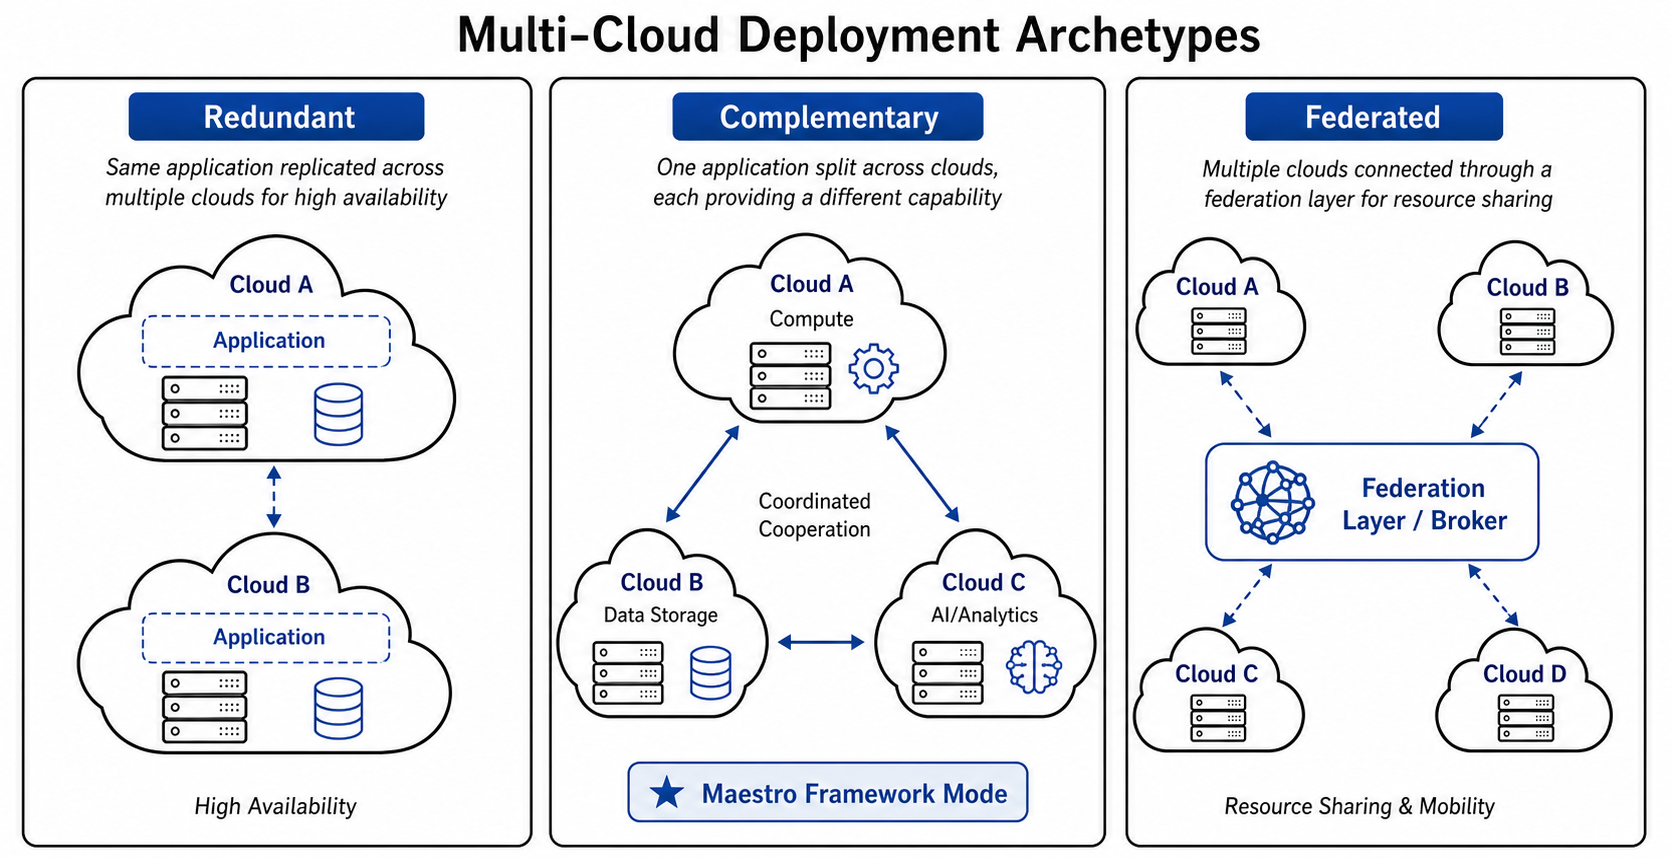
\includegraphics[width=0.85\textwidth]{5-Figures/Chapter2/multi-cloud-archetypes-maestro}
    \caption{Multi-cloud deployment archetypes - redundant, complementary, and federated strategies - as classified by Petcu~\cite{petcu2013interoperability}. The Maestro framework operates in complementary mode.}
    \label{fig:multi-cloud-archetypes-maestro}
\end{figure}

% TODO (author action): Replace the current AI-generated figure with an original, author-created diagram that accurately reflects the multi-cloud deployment archetypes as described by Petcu, following best practices for scientific illustration in LaTeX. Ensure the new figure is high quality, clearly labeled, and properly captioned.
%
% (Visible note for readers/evaluators: This figure is currently AI-generated and serves as a placeholder. The final submission will include an author-produced, publication-ready diagram.)
\todo[inline]{%
\textbf{[TODO]} Replace the current AI-generated figure with an original diagram%
}

%%------------------------------------------------------------
\subsection{Infrastructure as Code: Research Landscape and Practice}
\label{subsec:iac}

Infrastructure as Code (IaC) is the practice of expressing the configuration and
provisioning of computing infrastructure - virtual machines, networks, storage,
and managed services - as machine-readable, version-controlled source files
interpreted by a provisioning engine, rather than as manual operator procedures.
As cloud adoption accelerated, IaC became the primary mechanism for making
infrastructure reproducible, auditable, and amenable to code review and automated
testing.

\cite{rahman2019iac} conducted a systematic mapping study of the IaC research
landscape, identifying 32 peer-reviewed publications across six databases. They
distilled four topics defining the field's research agenda: (i) \emph{frameworks
and tools}, the design of provisioning engines and domain-specific languages;
(ii) \emph{use in practice}, adoption patterns and DevOps integration; (iii)
\emph{empirical studies}, analyses of defect prevalence, security flaws, and
quality metrics in IaC scripts; and (iv) \emph{testing}, validating
specifications prior to deployment~\cite{rahman2019iac}. A notable finding is that
empirical research and testing remained underexplored relative to tool-focused
contributions - a gap this dissertation partially addresses by empirically
evaluating the cost and operational consequences of IaC-governed multi-cloud
GenAI deployments.

Rahman et al.\ further observed that Ansible, Chef, Puppet, and Terraform were the
dominant tools, and that IaC research was growing with cloud adoption. Their
characterization of IaC as a practice that ``automatically configures system
dependencies and provisions local and remote instances'' captures its role in
Maestro~\cite{rahman2019iac}: the infrastructure layer is managed via
OpenTofu~\cite{closer2025maestro}, the Linux Foundation-governed fork of
HashiCorp Terraform, falling squarely within the tool-focused and empirical
categories Rahman et al.\ identify as core research vectors.

OpenTofu operates declaratively: practitioners specify the desired state of
resources - virtual networks, container registries, managed Kubernetes clusters,
secret stores, monitoring workspaces - and the engine computes a
dependency-ordered plan to converge actual state toward the target. The provider
model maps directly onto the multi-cloud architecture above: a single
configuration references Azure, AWS, and GCP provider plugins simultaneously,
each resource block scoped through namespace qualification. Because the provider
abstraction insulates declarations from the API differences documented by
Petcu~\cite{petcu2013interoperability}, operator-facing configuration remains
uniform regardless of host cloud - essential for a framework that spans multiple
providers.

The declarative approach further enables two properties relevant to this work's
objectives. It provides \emph{environment reproducibility}: the configuration
provisioning a staging environment can instantiate an identical topology in
production or a second region, eliminating configuration drift. It also
establishes a \emph{cost-attribution surface}: because every resource is declared
in versioned code, cost anomalies can be traced to specific changes through
commit history, supporting the FinOps disciplines of budget forecasting and spend
attribution central to this work~\cite{armbrust2010view, closer2025maestro}.

%%------------------------------------------------------------
%% SECTION: Cost Optimization
%%------------------------------------------------------------
\section{Cost Optimization}
\label{sec:cost-optimization}

The economic profile of LLM systems is dominated by inference costs that scale with the number of tokens processed, the model's capability tier, and the frequency of invocation. In multi-cloud deployments these costs accumulate across providers and workloads, making cost optimization a first-class architectural concern rather than a post-hoc adjustment \cite{armbrust2010view,petcu2013interoperability,closer2025maestro}. This section surveys five complementary technique classes - semantic caching, model cascades, prompt compression, reranking, and prompt caching - and the market context shaping their impact.

All of these mechanisms reduce a system's \emph{effective token cost}. Some reduce the tokens reaching a model (prompt compression, reranking), others reduce the number of model calls (semantic caching, prompt caching), and others reduce the marginal cost per call by routing to cheaper models (LLM cascades). In a multi-cloud setting they compose with provider-specific pricing to determine the realized cost of a workload \cite{gao2023ragsurvey,closer2025maestro}.

A unifying lens is \emph{tokenomics}: minimising token consumption relative to the semantic value delivered per inference call. The token is the atomic economic primitive of LLM systems - every capability is ultimately paid for in tokens whose price is governed by scaling-law dynamics \cite{brown2020gpt3}. Because the cost-accuracy trade-off can be shaped by architectural choice, as FrugalGPT demonstrates by achieving GPT-4-level accuracy at a fraction of its cost via adaptive routing \cite{chen2023frugalgpt}, tokenomics is a systems-design discipline, not merely a pricing concern. Market forces alone are insufficient: token prices have fallen substantially \cite{a16z2024llmflation}, yet total inference spend keeps growing as prompts and usage expand. Each technique surveyed here is thus a composable lever over a shared cost function, operating at one of three layers: the \emph{model layer} (cascade routing and dynamic model selection), the \emph{retrieval layer} (reranking and caching), and the \emph{representation layer} (prompt compression, output style, and data serialisation).

\subsection{Semantic Caching}
\label{subsec:semantic-caching}

Semantic caching is motivated by the observation that many production queries are not unique: users repeat, rephrase, or follow up on earlier requests. Traditional caches such as Redis match exact keys and cannot exploit semantic similarity, so even minor paraphrases miss. GPTCache addresses this with an open-source \emph{semantic} cache that stores responses and retrieves them via embedding-based similarity search rather than exact-string matching \cite{bang2023gptcache}.

Its architecture is straightforward. Incoming queries are encoded - along with stored queries and responses - into embeddings using a model compatible with vector databases such as Milvus or other ANN indexes \cite{bang2023gptcache}. A nearest-neighbour search determines whether a semantically similar query was already answered; if similarity exceeds a configurable threshold, the cached answer is returned. Only on a miss is the request forwarded to the LLM, and the new query–response pair inserted for future reuse \cite{bang2023gptcache}.

\begin{figure}[t]
    \centering
    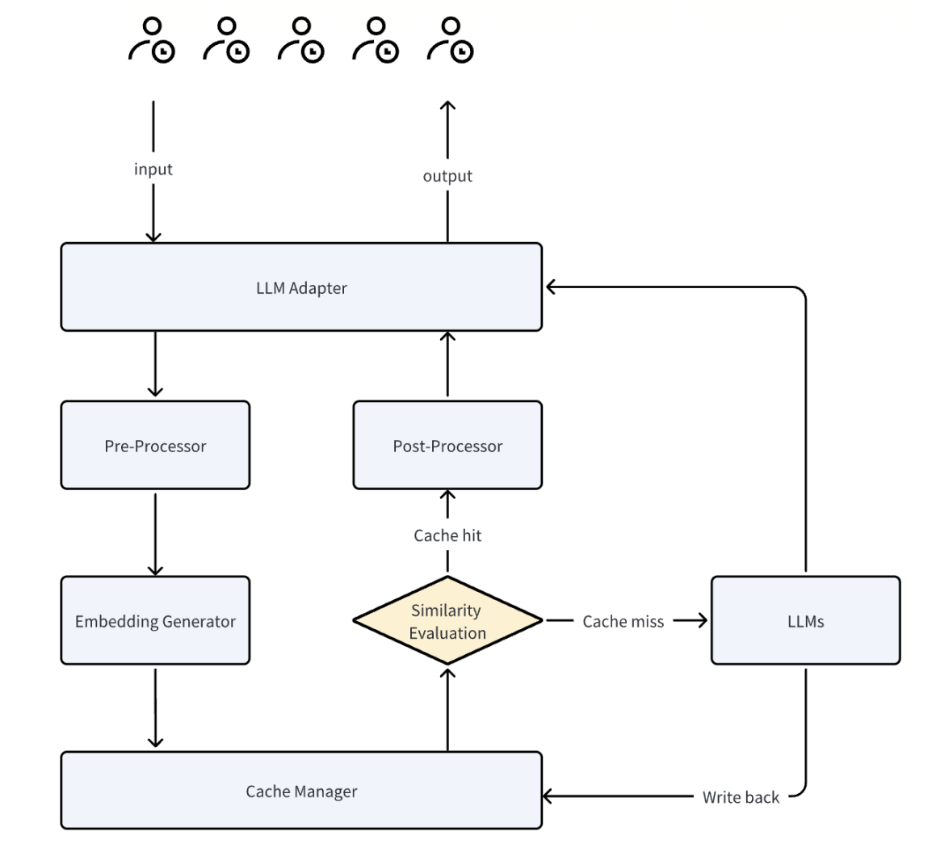
\includegraphics[width=\linewidth]{5-Figures/Chapter2/gptcache_architecture}
    \caption{Architecture of GPTCache as a semantic caching layer for LLM applications, showing the adapter, pre-processor, embedding generator, cache manager, similarity evaluator, and post-processor. Adapted from Bang et al. \cite{bang2023gptcache}.}
    \label{fig:gptcache-architecture}
\end{figure}

Empirically, when integrated with OpenAI's GPT services, cache hits increase response speed by 2–10$\times$ while insulating the application from network and provider-side latency spikes \cite{bang2023gptcache}. Because an embedding lookup costs negligibly compared to a full LLM call, even a modest hit rate yields tangible API savings - particularly for enterprise assistants, FAQ bots, and RAG systems where queries repeat strongly across tenants and time \cite{bang2023gptcache,closer2025maestro}.

In the multi-cloud framework studied here, semantic caching aligns naturally with existing RAG infrastructure: the system already computes embeddings for retrieval and indexing, so backing a semantic cache requires minimal change. Deployed as a cross-cutting concern in the LLM gateway, it intercepts repeated queries before they reach any provider, reducing both cost and latency across clouds \cite{closer2025maestro,liu2022llamaindex}.

\subsection{LLM Cascades}
\label{subsec:llm-cascades}

Where semantic caching reduces redundant \emph{calls}, LLM cascades target \emph{which} model is invoked when a call is necessary. FrugalGPT studies how to route queries across a portfolio of models to minimize cost subject to accuracy constraints, on the premise that not all requests need the most capable (and expensive) model: many can be handled by smaller models, provided the system can distinguish "easy" from "hard" queries \cite{chen2023frugalgpt}.

FrugalGPT proposes several routing strategies: rule-based routing on query features, learned policies predicting which model will answer correctly, and multi-step cascades where a cheap model answers first and escalates only if its answer is judged unsatisfactory \cite{chen2023frugalgpt}. Such cascades reduce inference cost by 50–98\% while matching the best single model's accuracy; in some configurations FrugalGPT even exceeds GPT-4 accuracy at equal or lower cost by combining multiple models \cite{chen2023frugalgpt}.

This connects to scaling-law and alignment research. Larger models generally perform better but at higher per-token cost \cite{brown2020gpt3}, while alignment work such as InstructGPT shows smaller, well-aligned models can outperform larger unaligned ones on preference metrics \cite{ouyang2022instructgpt}. FrugalGPT leverages both by routing most traffic to small, cheap models and reserving larger models for edge cases that benefit from their capacity \cite{chen2023frugalgpt,ouyang2022instructgpt}.

In a multi-cloud framework, cascades can be realized at the LLM gateway, which exposes a single logical endpoint while internally routing among on-premise open-weight models (e.g., Llama 2), mid-tier cloud APIs, and frontier proprietary models, per a policy informed by query characteristics, historical performance, and business priorities \cite{touvron2023llama2,closer2025maestro}. This turns model choice from static configuration into a dynamic optimization over latency, accuracy, and cost, tunable per tenant or workload.

\begin{figure}[t]
    \centering
    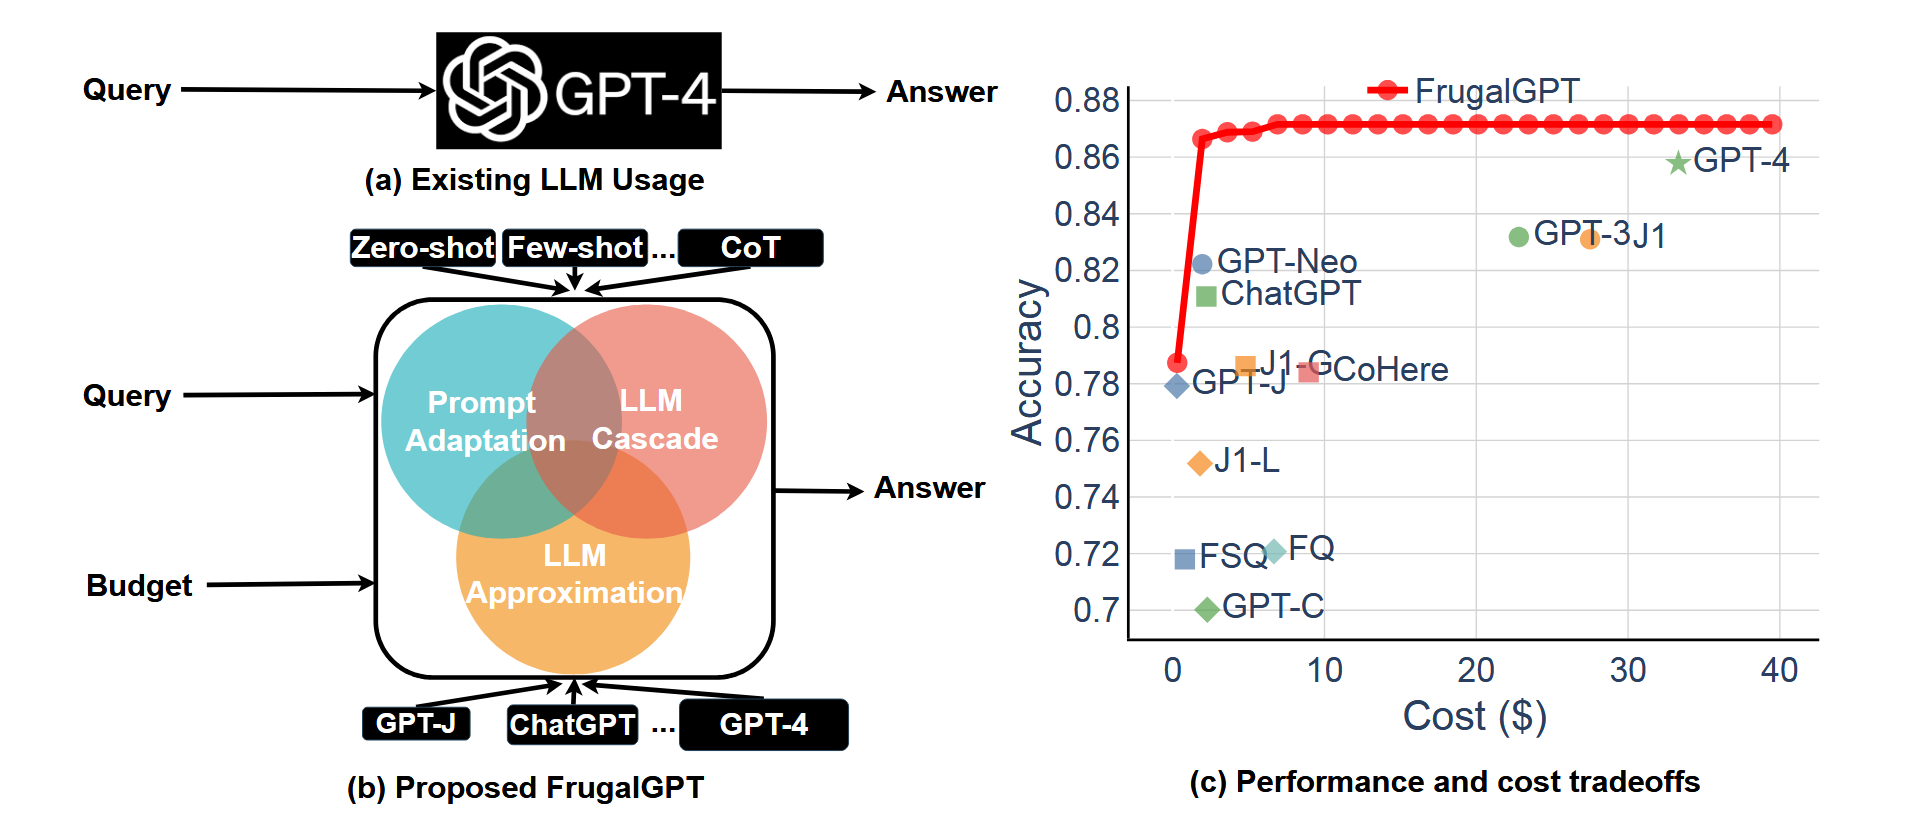
\includegraphics[width=\linewidth]{5-Figures/Chapter2/frugalGPT}
    \caption{Overview of cost-reduction strategies in FrugalGPT, including prompt adaptation, LLM approximation, and LLM cascade. Adapted from Chen et al. \cite{chen2023frugalgpt}.}
    \label{fig:frugalgpt-strategies}
\end{figure}

\subsection{Prompt Compression}
\label{subsec:prompt-compression}

Prompt compression addresses a different cost driver: the number of tokens processed per inference. Transformer attention scales quadratically with sequence length, so longer prompts cost more and are slower \cite{vaswani2017attention,brown2020gpt3}. In enterprise workflows, prompt length is often dominated not by the user's query but by system instructions, conversation history, and retrieved RAG context \cite{gao2023ragsurvey,closer2025maestro}.

Research on prompt compression explores how much input can be removed without materially degrading performance, ranging from heuristic truncation and summarization to learned models that identify salient segments. The LLM-in-a-Flash work by Jin et al.\ focuses on hardware-level optimizations - storing weights on flash memory and using windowing and row–column bundling to reduce data transfer - but illustrates a broader point: much LLM inference cost stems from unnecessary data movement and redundant processing, at both hardware and token levels \cite{jin2023llminflash,vaswani2017attention}. Their cost model accounts for flash characteristics: windowing reuses previously activated neurons to reduce reads, and row–column bundling increases read contiguity. Together these enable running models up to twice the size of available DRAM, with reported 4–5$\times$ CPU and 20–25$\times$ GPU speed-ups over naive loading \cite{jin2023llminflash}.

The key analogy for this dissertation is that token-level prompt compression plays the same role at the software layer that windowing and bundling do at the hardware layer: both reduce the information handled per request. In practice, a compression step inserted between retrieval and generation summarizes or filters retrieved passages and history before the LLM call, significantly reducing token usage without sacrificing answer quality, especially in knowledge-intensive tasks with verbose documents \cite{gao2023ragsurvey,closer2025maestro}.

The most academically grounded software-layer approach is the LLMLingua family. LLMLingua (Jiang et al.,\ EMNLP 2023) uses a small surrogate model - GPT-2 or LLaMA-7B - to score each token's saliency via conditional perplexity \cite{jiang2023llmlingua}: tokens highly predictable from context carry little unique information and can be removed with minimal impact. Its pipeline has three stages: a budget controller setting the global compression ratio, iterative token-level pruning of low-saliency tokens, and an instruction-tuning alignment stage recovering any quality loss. Empirically, it achieves up to 20$\times$ compression while preserving the factual content needed for correct answers \cite{jiang2023llmlingua}. LLMLingua-2 (Pan et al.,\ 2024) reformulates compression as token classification \cite{pan2024llmlingua2}: instead of unidirectional perplexity, it trains a bidirectional encoder on data distilled from GPT-4, making retention decisions from both left and right context - task-agnostic, faster at inference, and more faithful than the perplexity-based approach \cite{pan2024llmlingua2}. Both exploit the same gap: a large fraction of tokens in any well-formed prompt are consumed by grammatical predictability - articles, auxiliary verbs, hedging - rather than factual content. Eliminating this overhead removes tokens whose marginal semantic value is near zero, a principle revisited at the representation layer in Section~\ref{subsec:tokenomics-practice}.

\begin{figure}[t]
    \centering
    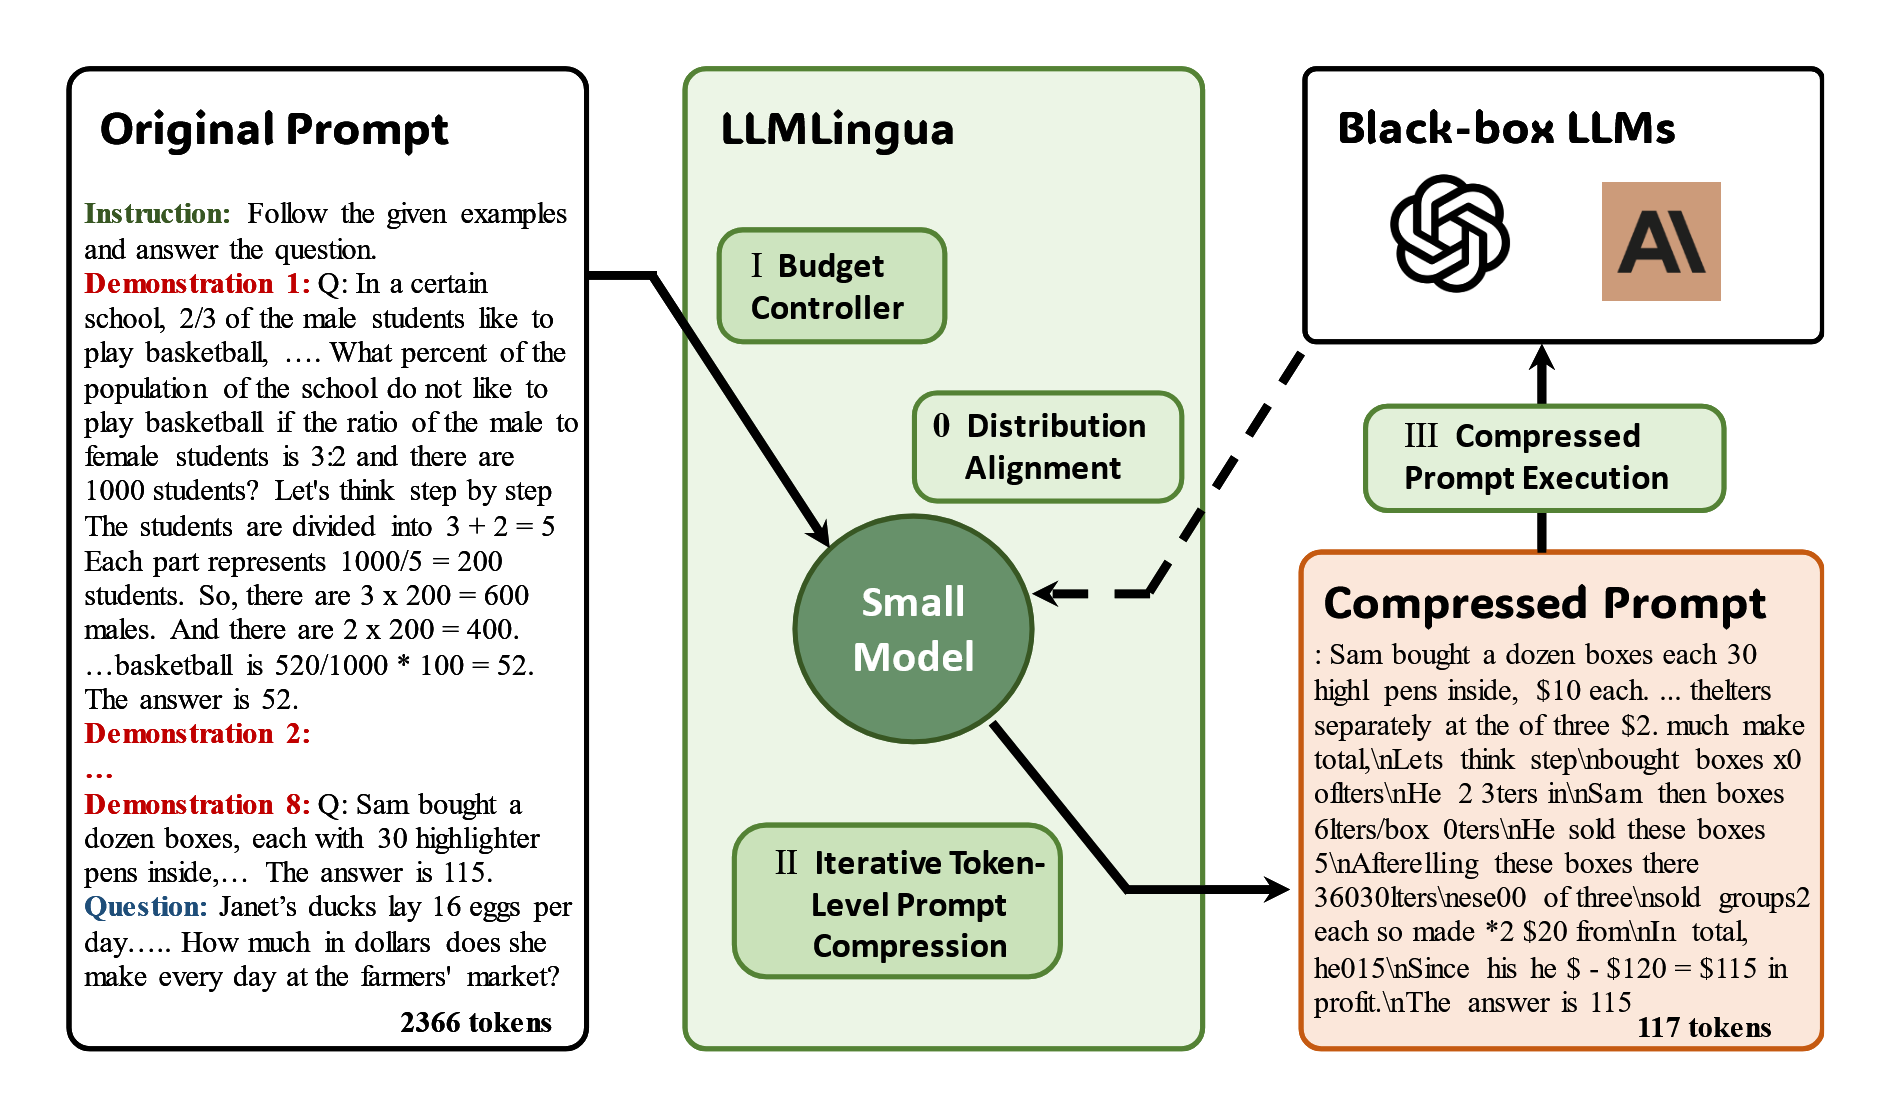
\includegraphics[width=\linewidth]{5-Figures/Chapter2/llmlingua}
    \caption{The LLMLingua coarse-to-fine prompt compression framework, comprising a budget controller, iterative token-level compression, and a distribution alignment stage. The small surrogate model scores token saliency via conditional perplexity; low-saliency tokens are iteratively removed before the compressed prompt is forwarded to the target LLM. Adapted from Jiang et al. \cite{jiang2023llmlingua}.}
    \label{fig:llmlingua-pipeline}
\end{figure}

\subsection{Reranking Efficiency}
\label{subsec:reranking-efficiency}

Reranking improves retrieval efficiency and quality, which indirectly affects cost by shaping how much context enters the prompt. In naive RAG, the top-$k$ documents from a vector search are concatenated with the query and fed to the LLM - brittle because too small a $k$ omits relevant information while too large a $k$ yields long, noisy prompts that raise cost and hallucination risk \cite{lewis2020rag,gao2023ragsurvey}.

Advanced RAG adds a reranking stage: an initial dense retriever proposes a candidate set, and a more expensive cross-encoder re-scores it to select a smaller, higher-precision subset for the prompt \cite{gao2023ragsurvey}. This shifts cost from the generator to the retriever - spending controlled compute upfront to filter rather than asking the LLM to ignore irrelevant passages in a long prompt. Measured in effective token cost, reranking can therefore be cheaper than inference-time reasoning over large contexts.

In this work, reranking can be a dedicated microservice in the RAG subsystem: the vector store returns a larger candidate set (e.g., $k=50$), reranked by a cross-encoder such as a Sentence-BERT variant fine-tuned for passage relevance, before selecting a smaller subset (e.g., $m=5$–$10$) for the prompt \cite{reimers2019sbert,liu2022llamaindex}. This improves evidence quality while keeping prompt size - and thus generation cost - under control \cite{gao2023ragsurvey,closer2025maestro}.

\subsection{Prompt Caching}
\label{subsec:prompt-caching}

Prompt caching is a complementary mechanism recently introduced at the API layer by major providers: repeated prompt prefixes - long system prompts, policy text, or shared instructions - are cached provider-side and billed at a discount when reused. Anthropic's MCP ecosystem and related documentation describe prompt caching as part of a broader effort to standardize how hosts and tools expose context, including efficient reuse of stable prompt templates \cite{anthropic2024mcp,modelcontextprotocol2024}.

Prompt caching differs from semantic caching in two respects. It operates on \emph{exact} prefix reuse rather than semantic similarity - the cached segment must be identical for the discount to apply - and it does not bypass inference but makes the repeated portion cheaper while processing the new suffix at full price. This is attractive for enterprise assistants where much of each prompt is fixed instructions or policies that change rarely relative to user queries \cite{anthropic2024mcp,modelcontextprotocol2024}.

Prompt-caching support varies across providers, but the design principle is constant: the orchestration layer should separate stable prompt components from dynamic ones so repeated prefixes are reused across requests and sessions. Combined with semantic caching and cascades, prompt caching captures both vendor-side and application-side reuse, jointly reducing latency and cost without compromising behavior \cite{closer2025maestro,chase2022langchain}.

\subsection{Market Context and LLMFlation}
\label{subsec:market-context}

The urgency of cost optimization is shaped by LLM pricing dynamics. Sardana and Frankle introduce ``LLMflation'' to describe the rapid decline in inference costs, arguing that token prices have dropped by orders of magnitude for comparable capability as infrastructure, hardware, and model efficiency improved \cite{a16z2024llmflation}; token price indices report similar reductions across proprietary and open-weight ecosystems.

Lower unit prices do not automatically yield lower total spend. As LLMs become cheaper and more capable, organizations expand usage, apply models to more workflows, and supply more context per query, especially in RAG and agentic settings \cite{gao2023ragsurvey,closer2025maestro}. Demand growth and prompt-length inflation can outpace price cuts, raising absolute cost despite lower per-token rates - mirroring cloud computing, where falling resource prices often coincided with rising expenditure from workload expansion \cite{armbrust2010view,petcu2013interoperability}.

The literature therefore argues that cost optimization must be embedded in system architecture rather than treated as a transient concern to be ``solved'' by future price cuts. Semantic caching, cascades, prompt compression, reranking, and prompt caching remain valuable even as prices fall, because they target structural cost drivers: repeated queries, over-provisioned capacity, unnecessary tokens, and inefficient retrieval \cite{bang2023gptcache,chen2023frugalgpt,gao2023ragsurvey,a16z2024llmflation}. In a multi-cloud environment, these levers also interact with placement and portability decisions that determine how workloads are distributed across providers and pricing regimes \cite{petcu2013interoperability,closer2025maestro}.

\begin{figure}[t]
    \centering
    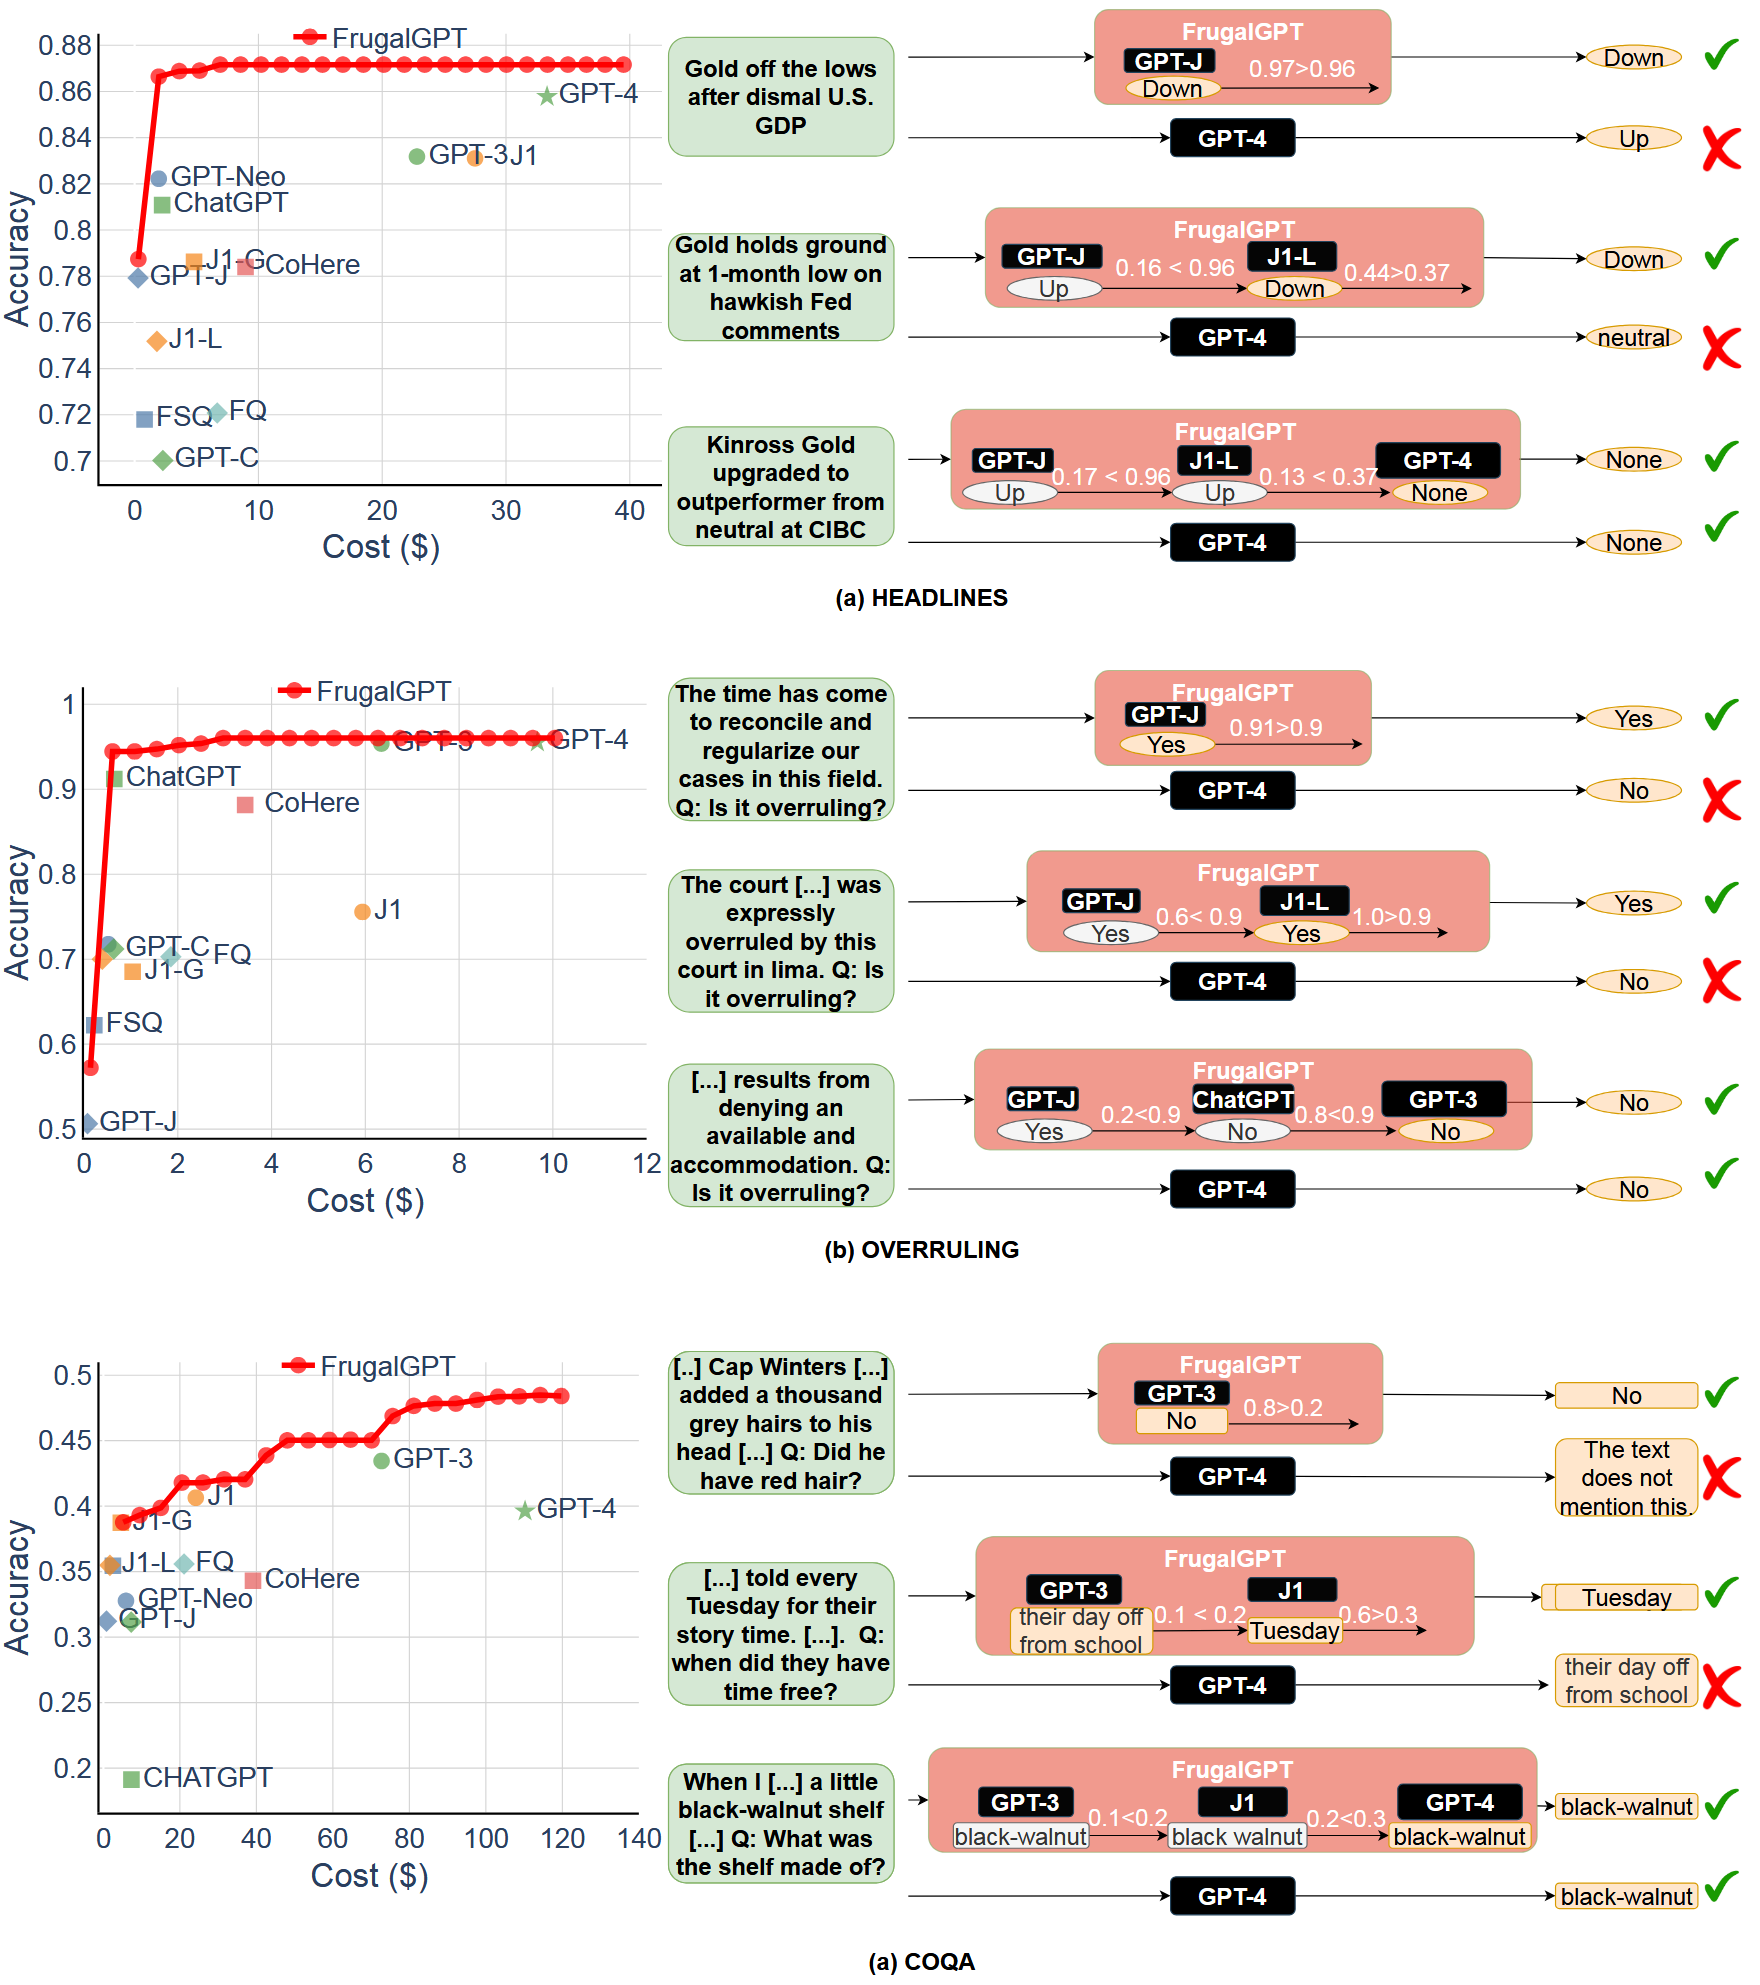
\includegraphics[width=\linewidth]{5-Figures/Chapter2/frugalgpt_tradeoff}
    \caption{Accuracy and cost tradeoff achieved by FrugalGPT, showing that adaptive LLM cascades can reduce inference cost while maintaining or improving task performance. Adapted from Chen et al. \cite{chen2023frugalgpt}.}
    \label{fig:frugalgpt-tradeoff}
\end{figure}

\subsection{Tokenomics in Practice: Representation and Style as Cost Levers}
\label{subsec:tokenomics-practice}

Beyond model- and retrieval-layer optimisations, token consumption is shaped by choices that precede or follow the model call: the format in which structured data is serialised into the prompt and the verbosity of the requested output. These representation-layer decisions are less studied than caching or routing, but empirical evidence suggests savings comparable to software-layer compression.

One practitioner contribution is TOON (Token-Oriented Object Notation), a compact drop-in replacement for JSON in LLM prompts \cite{toon2025}. It exploits a structural inefficiency in JSON: for tabular payloads, every row repeats the full key set and delimiters, most of which encode schema rather than data. TOON declares column headers once and encodes rows as tab-delimited values, retaining relational structure while removing per-row key verbosity. Practitioner benchmarks report 30–60\% token reductions on flat tabular structures without semantic loss \cite{toon2025}. This is consequential for enterprise RAG systems injecting structured business data - product catalogues, API schemas, entity metadata - as JSON, where key repetition can be a significant fraction of prompt length.

A complementary practitioner finding is Caveman Compression \cite{brussee2025caveman}, predicated on the observation that LLMs can produce factually equivalent responses in a telegraphic register omitting articles, auxiliary verbs, and hedging, without degrading accuracy or actionability. The original Claude Code skill by Brussee (2025) achieved roughly 75\% output token reduction on structured tasks \cite{brussee2025caveman}, while a distillation by Guzik (2026) reduced the meta-instruction from 552 to 85 tokens while preserving 14–21\% savings over a ``Be concise'' baseline \cite{guzik2026cavemanmicro}. Its mechanistic basis matches the LLMLingua framing of Section~\ref{subsec:prompt-compression}: both exploit the gap between the budget consumed by predictable surface forms and that strictly needed for the factual payload. The distinction is directional - LLMLingua removes predictable tokens from the \emph{input}, Caveman Compression from the \emph{output} - but both target the same redundancy. These findings originate in practitioner benchmarks rather than peer-reviewed studies, and are included as empirical evidence of the representation-layer effect and motivation for formal investigation.

The three-layer tokenomics model can now be stated explicitly. At the \emph{model layer}, cascade routing and dynamic model selection - as formalised by FrugalGPT \cite{chen2023frugalgpt} - invoke expensive frontier models only when warranted. At the \emph{retrieval layer}, semantic caching \cite{bang2023gptcache}, prompt caching, and reranking prevent redundant calls and filter irrelevant context. At the \emph{representation layer}, compression such as LLMLingua \cite{jiang2023llmlingua}, format optimisations such as TOON \cite{toon2025}, and output style control such as Caveman Compression \cite{brussee2025caveman} eliminate tokens whose marginal semantic contribution is low relative to their billing weight. This taxonomy frames the engineering contributions of this dissertation, in which the Maestro improvements address cost levers at all three layers within a unified multi-cloud architecture.

\begin{figure}[t]
    \centering
    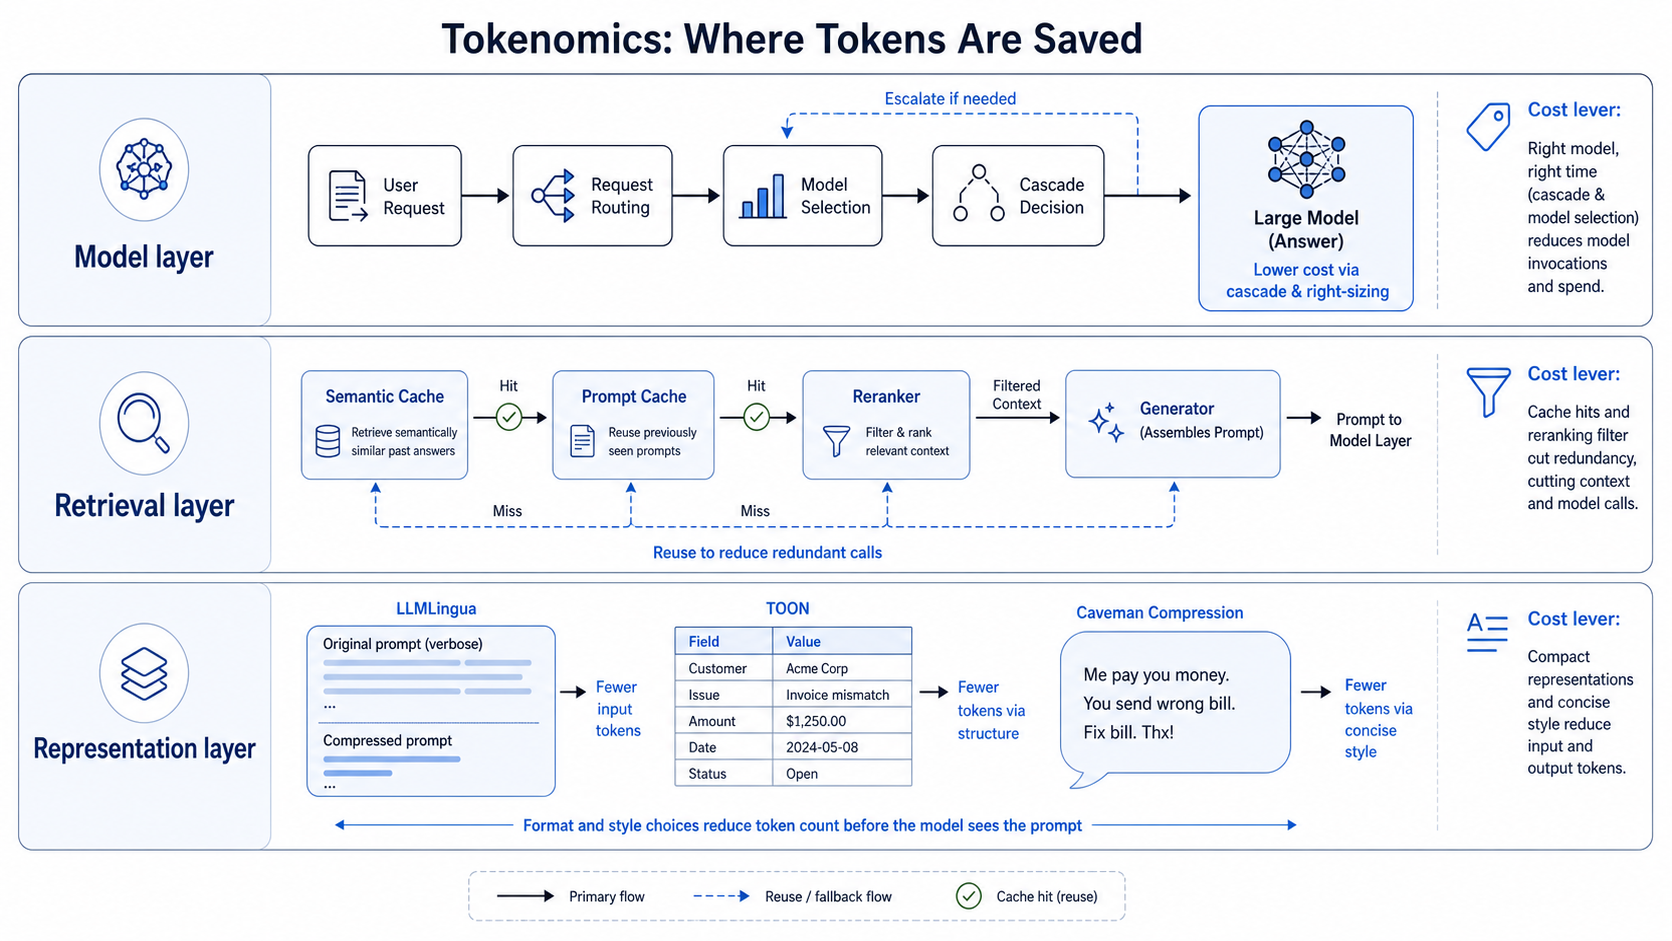
\includegraphics[width=\linewidth]{5-Figures/Chapter2/tokenomics-3-layers}
    \caption{Three-layer tokenomics model for cost optimization in enterprise GenAI systems. The model layer controls cascade routing and dynamic model selection; the retrieval layer governs semantic caching, prompt caching, and reranking; the representation layer encompasses software compression (LLMLingua), format optimisation (TOON), and output style control (Caveman). Each layer targets a structurally distinct source of token consumption.}
    \label{fig:tokenomics-layers}
\end{figure}

%%------------------------------------------------------------
%% SECTION: GenAI Operations and Governance
%%------------------------------------------------------------

\section{GenAI Operations and Governance}
\label{sec:genai-ops-governance}

Deploying Generative AI systems into production introduces operational challenges that extend well beyond traditional software engineering. While earlier sections examined the architectural components of RAG pipelines and the cost dynamics of LLM inference, this section addresses the orthogonal question of how such systems are governed, monitored, and sustained over time. The central argument is that operational governance is not an optional layer atop a working system but a structural requirement whose absence compounds into systemic risk - a perspective grounded in a body of literature that has progressively refined the vocabulary and methodology for managing ML systems in production.

\subsection{The Technical Debt Perspective on ML Operations}

The conceptual foundation for these governance challenges was established by \cite{sculley2015debt}, whose seminal work catalogued the \textit{hidden technical debt} that accumulates in ML pipelines. ML code typically constitutes a small fraction of the system; the dominant cost lies in surrounding infrastructure - data ingestion, feature engineering, serving, monitoring, and configuration management. This infrastructure is subject to \textit{boundary erosion}, whereby coupling between data distributions, model behaviours, and downstream consumers degrades silently over time, without explicit failures.

Particularly relevant to RAG is the CACE principle - ``Change Anything, Changes Everything'' - describing how altering a single upstream artefact, such as an embedding model or chunking strategy, may propagate unexpected behaviour through the system \cite{sculley2015debt}. In a production RAG framework such as Maestro this entanglement is amplified: it integrates a continuously evolving knowledge base, a swappable retrieval layer, and a provider-agnostic LLM interface, each a potential source of silent degradation. Sculley et al.\ thus provide the normative justification for this thesis's governance objectives: without systematic instrumentation, evaluation, and operational discipline, technical-debt accumulation in GenAI systems is not merely possible but inevitable.

\subsection{Evaluating RAG Pipeline Quality in Production}

A RAG governance framework is only as rigorous as its evaluation methodology. Classical metrics such as BLEU and ROUGE are inadequate for retrieval-augmented outputs, evaluating surface-level lexical overlap rather than factual faithfulness or contextual relevance \cite{es2023ragas}. To address this, \cite{es2023ragas} introduced RAGAS (\textit{Retrieval Augmented Generation Assessment}), a reference-free framework that assesses RAG pipelines along multiple quality dimensions without manually annotated ground truth.

RAGAS decomposes pipeline quality into four metrics: \textit{faithfulness} (how far answers are grounded in retrieved context), \textit{answer relevance} (whether the response addresses the question), \textit{context precision} (whether retrieved passages focus on relevant information), and \textit{context recall} (whether retrieval covers the information needed for a correct answer) \cite{es2023ragas}. Computed via an LLM-as-judge paradigm, they enable automated, scalable evaluation embeddable directly into CI and monitoring pipelines. RAGAS is the methodological basis for the output-quality objective - O3 in this thesis - and the instrumentation through which Maestro's retrieval and generation quality is tracked in production.

\subsection{RAGOps: Operationalising the Dual Lifecycle}

The rise of RAG as the dominant enterprise LLM paradigm has surfaced operational challenges that existing LLMOps practices cannot address. Xu et al. \cite{xu2025ragops} introduce \textit{RAGOps} to characterise the discipline required to manage RAG pipelines in production, arguing that such systems have a dual lifecycle: an \textit{LLM lifecycle} governing model versioning, prompt management, and inference configuration; and a \textit{data lifecycle} governing the evolution, quality, and freshness of the external knowledge base.

This framing is consequential for design. In a conventional deployment the model artefact is the primary unit of management, stable between updates. In a RAG system the knowledge base changes continuously - documents are ingested, revised, or deprecated; embedding distributions shift as indexing evolves; and retrieval relevance may degrade independently of any model change \cite{xu2025ragops}. Xu et al. \cite{xu2025ragops} characterise RAGOps concerns via a 4+1 model view spanning logical, process, development, and physical dimensions. Applied to Maestro, this motivates automated mechanisms for knowledge-base staleness, embedding index versioning, and retrieval-quality monitoring - capabilities not routinely addressed by LLMOps tooling built for static deployments. They additionally report that roughly 60\% of enterprise LLM deployments incorporate retrieval augmentation, underscoring the urgency of the discipline.

\subsection{Financial Governance: The FinOps Lifecycle for AI}

Operational governance of GenAI systems also has an economic dimension. Token-priced inference is more dynamic and usage-dependent than the resource-reservation models typical of classical cloud workloads, and without deliberate financial governance, LLM systems are susceptible to overruns from prompt inefficiency, suboptimal routing, or unconstrained retrieval. The FinOps Foundation has extended its cloud financial management framework to these AI dynamics, defining a three-phase cycle: \textit{Inform}, \textit{Optimize}, and \textit{Operate} \cite{finops2024ai}.

The \textit{Inform} phase establishes visibility into AI expenditure by instrumenting token usage, call frequency, and cost per query. The \textit{Optimize} phase uses this visibility to implement improvements - model downsizing for low-complexity queries, semantic caching, prompt compression, and retrieval efficiency. The \textit{Operate} phase embeds these into ongoing practice, establishing cross-functional accountability between engineering, product, and finance and closing the loop iteratively \cite{finops2024ai}. The cycle is continuous by design: cost governance is positioned not as a one-time exercise but as a persistent discipline integrated into deployment and monitoring. This informs the cost-efficiency objective - O2 in this thesis - and provides the structure within which the earlier cost-reduction techniques are situated as components of a managed, accountable process rather than isolated interventions.

\subsection{Synthesis: Towards a Governed GenAI Operations Model}

The four perspectives converge on a unified thesis: deploying a GenAI system is far less demanding than governing it sustainably in production. Sculley et al. \cite{sculley2015debt} established the structural sources of operational risk; Xu et al. \cite{xu2025ragops} extended this to the dual-lifecycle complexity of RAG; Es et al. \cite{es2023ragas} provided the evaluation instrumentation for quality governance; and the FinOps Foundation supplied the financial framework within which quality and cost objectives are managed accountably.

Together these define a layered governance model for production RAG systems, progressing from \textit{structural risk awareness} (Sculley et al.) through \textit{architectural discipline} (RAGOps) to \textit{quality measurement} (RAGAS) and \textit{financial accountability} (FinOps). Maestro is positioned as an instantiation of these principles in an enterprise multi-cloud context. The objectives O2 and O3 - cost efficiency and output quality assurance - correspond directly to the Optimize and Inform–Operate dimensions, grounding this work's empirical contributions in an established, industry-validated governance architecture.